\documentclass[conference]{IEEEtran}
\IEEEoverridecommandlockouts
% The preceding line is only needed to identify funding in the first footnote. If that is unneeded, please comment it out.
%Template version as of 6/27/2024

\usepackage{cite}
\usepackage{amsmath,amssymb,amsfonts}
\usepackage{algorithmic}
\usepackage{graphicx}
\usepackage{textcomp}
\usepackage{xcolor}
\usepackage[utf8]{inputenc}
\usepackage[T1]{fontenc}
\usepackage{array}
\usepackage{adjustbox}
\def\BibTeX{{\rm B\kern-.05em{\sc i\kern-.025em b}\kern-.08em
    T\kern-.1667em\lower.7ex\hbox{E}\kern-.125emX}}
\begin{document}

\title{AMEND: Asymmetric Cleaning of Minority-to-Majority Label Errors in Small, High-Dimensional Imbalanced Datasets}

\author{\IEEEauthorblockN{1\textsuperscript{st} Mohammed Adel Omer}
\IEEEauthorblockA{\textit{Climate Change Information Center,} \\
\textit{Renewable Energy \& Expert System}\\
Cairo, Egypt \\
m.adel.omer@gmail.com}
\and
\IEEEauthorblockN{2\textsuperscript{nd} Khaled Tawfik Wassif}
\IEEEauthorblockA{\textit{Department of Computer Science} \\
\textit{Faculty of Computers and Artificial Intelligence}\\
\textit{Cairo University}\\
Cairo, Egypt \\
kwassif@fci-cu.edu.eg}
\and
\IEEEauthorblockN{3\textsuperscript{rd} Samar Hesham}
\IEEEauthorblockA{\textit{Department of Computer Science} \\
\textit{Faculty of Computers and Artificial Intelligence}\\
\textit{Cairo University}\\
Cairo, Egypt \\
samar@fci-cu.edu.eg}
}

\maketitle

\begin{abstract}
In small, high-dimensional, imbalanced datasets the most damaging label error is a genuine minority case recorded as the common class. The case vanishes from the rare class, and a cleaner that then deletes suspect minority samples discards information that cannot be recovered. This paper studies asymmetric cleaning aimed at these minority-to-majority errors. AMEND deletes suspect samples only when they carry the majority label, quarantines suspect minority-labelled samples at low weight instead of deleting them, and ranks suspects by combining neighbour-label disagreement with local subspace agreement. On 13 binary datasets with 50 to 253 samples and 2000 to 22 283 features, evaluated with ten repetitions of stratified five-fold cross-validation and five classifiers, AMEND raised F1 over no cleaning at every minority-to-majority noise rate from 5\% to 40\% (Holm-adjusted p $\le $ 0.027), matched confident learning (CL) and cleaned about seven times faster. Controls identify the asymmetry as the active ingredient. In this regime AMEND's removals beat random majority undersampling of the same size for three of five classifiers, a variant allowed to delete minority samples was worse for all five, and neither the soft weights nor the subspace term improved on simpler alternatives. When the least confident minority samples were flipped, AMEND also exceeded CL (+0.036 F1 at 30\% noise). Outside this regime the rule offers little: CL detects wrong labels far more accurately, AMEND's gains under uniform noise match those of random undersampling, and it loses F1 when majority labels are flipped to the minority class.
\end{abstract}

\begin{IEEEkeywords}
label noise, asymmetric data cleaning, minority-to-majority label errors, class imbalance, instance selection, high-dimensional data, small-sample learning
\end{IEEEkeywords}

\section{Introduction}\label{sec:introduction}

Supervised learners assume that training labels are correct, and label noise degrades both the classifiers trained on the data and the conclusions drawn from them \cite{frenay2014,song2023}. Wrong labels are common even in curated benchmarks: an audit of ten widely used test sets found label errors in all of them, enough to change which model appears to be the best \cite{northcutt2021pervasive}. The damage is uneven when classes are imbalanced \cite{he2009,johnson2019}. If a dataset has 25 positive cases and three are recorded as negatives, 12\% of the rare class has moved into the majority, and a learner trained on those labels sees a smaller and partly self-contradictory minority.

This paper is concerned with a setting where that problem is acute and the usual remedies are hardest to apply: datasets with tens to a few hundred samples, thousands of features and a rare class of clinical or operational interest, as in gene-expression studies. Two properties of this setting shape the design of a cleaner. First, every sample of the rare class is precious. A minority case that has already been mislabelled as the majority is invisible to the analyst; if a cleaner then deletes a genuine minority sample, that information is lost for good, and with 7 to 91 minority samples per dataset a few such deletions matter. The asymmetry is not only statistical but practical, since in screening and diagnosis a missed positive usually costs more than a false alarm. Second, with far more features than samples, every local estimate is made from a handful of points in a very high-dimensional space, so a cleaner must control both its statistical and its computational dependence on the number of features.

Existing approaches address one side of this or the other. Classifier-based filters --- consensus filtering \cite{brodley1999}, instance hardness \cite{smith2014}, area under the margin \cite{pleiss2020} and confident learning \cite{northcutt2021confident} --- infer wrong labels from held-out model predictions, which is powerful but depends on a model that can be fitted reliably when a class has only a few dozen members, and their pruning is symmetric in the sense that a suspect minority sample is discarded like any other. Neighbourhood editing rules such as ENN and AllKNN \cite{wilson1972,tomek1976} need no trained model but judge a sample only by the labels of its neighbours, and in our experiments they discarded a third or more of the training data. Neither family treats the rare class differently, and neither returns anything softer than a keep-or-delete verdict.

The central contribution of this paper is an asymmetric cleaning rule aimed at that error, and a test of whether the asymmetry, rather than anything else in the cleaner, is what helps. AMEND (Asymmetric Minority-protecting Editing of Noisy Data) deletes a suspect sample only when it carries the majority label, which is where minority-to-majority errors hide. Suspect minority-labelled samples are quarantined at low weight rather than deleted and are reinstated if they cohere with confident minority samples, and borderline samples in either class receive intermediate weights. Suspects are ranked by a score that mixes neighbour-label disagreement with the agreement between a sample's local principal subspace and those of its same-label neighbours. Every structural parameter (neighbourhood size, local rank, projection width, flagging threshold) is set from the data, and a Johnson--Lindenstrauss projection \cite{johnson1984} bounds the work per sample in the number of features, so the same configuration runs on 2000 and on 22 283 features without retuning. We evaluate each component separately. The asymmetric removal rule is the part the evidence supports; the geometric score and the soft weights, which we expected to matter, add little, and we report that result in full.

\begin{itemize}
\item An asymmetric cleaning rule for minority-to-majority label errors, in which deletion is confined to majority-labelled samples and suspect minority-labelled samples are quarantined and can be rescued, with a complete description of AMEND: its automatic choice of neighbourhood size, local rank, projection width and threshold, and its cost in the number of features (Section III).
\item An evaluation on 13 small, high-dimensional binary datasets under three class-conditional noise models at six rates and two instance-dependent noise models at four rates, with five classifiers and five established cleaners including confident learning, which is also run with each classifier as its own base model, plus a threshold-free ranking analysis, a minority-size sweep, an ablation and runtime measurements (Sections IV and V).
\item Evidence that isolates the asymmetry: random majority undersampling matched per fold to AMEND's removals, AMEND's removal and weighting applied separately, and a fully symmetric variant that may delete minority samples; a sweep of the agree-weight $w$ that tests the subspace term against neighbour-label disagreement in the same projected space and at the same $k$; and an audit of AMEND's internal state (Sections V-F, V-I and V-K).
\item A direct analysis of the high-dimensional regime (Section V-M): how AMEND's standing relative to confident learning varies with the feature-to-sample ratio, and how its runtime responds to the number of features.
\item An evidence-graded account of the results that separates Holm-corrected findings from observations (Table XVII) and keeps noise-detection accuracy apart from downstream classification, identifying where AMEND helps (minority$\rightarrow $majority and minority instance-dependent noise; random forests; conservative removal whose selection beats matched random undersampling in the target regime; speed on wide data) and where it does not (detection and ranking against confident learning, uniform noise, majority$\rightarrow $minority noise, ROC-AUC, false positives, the contribution of the subspace term and the response of the threshold to the noise level).
\end{itemize}

\section{Related work}\label{sec:related-work}

\subsection{Label noise: robust learning and data cleansing}\label{sec:label-noise-robust-learning-and-data-cleansing}

Frénay and Verleysen \cite{frenay2014} divide responses to label noise into noise-robust learners, noise-tolerant models and data cleansing; AMEND belongs to the third group. The recent literature is dominated by the first two, mostly for deep networks: robust loss functions \cite{ghosh2017,zhang2018}, loss correction using an estimated transition matrix \cite{patrini2017}, sample-selection schemes that train two networks and let each teach the other \cite{han2018} or learn a curriculum over samples \cite{jiang2018}, and semi-supervised treatments that relabel suspect samples rather than discard them \cite{li2020}. Song et al. \cite{song2023} survey this body of work. These methods assume a training regime that does not exist in our setting: they need many samples, gradient-based training over many epochs and per-epoch loss statistics, whereas a 50-sample gene-expression dataset is typically handled with a support vector machine or a random forest. The idea we do borrow from that literature is that a suspect sample can be down-weighted or relabelled instead of deleted \cite{li2020}, which is what AMEND's quarantine and soft weights implement for classical learners.

\subsection{Model-based label-error detection}\label{sec:model-based-label-error-detection}

Cleansing methods identify wrong labels from the behaviour of a trained model. Brodley and Friedl \cite{brodley1999} used majority and consensus filters over cross-validated classifiers. Instance hardness \cite{smith2014} estimates how often a sample is misclassified across learners, and the InstanceHardnessThreshold implementation in imbalanced-learn \cite{lemaitre2017} discards samples whose cross-validated probability for their own class is low. Area Under the Margin \cite{pleiss2020} ranks samples by their average margin during training and calibrates the cut-off with samples given deliberately wrong labels. Confident learning (CL) \cite{northcutt2021confident} estimates the joint distribution of observed and true labels from out-of-sample predicted probabilities and prunes accordingly, with theoretical guarantees under class-conditional noise and a widely used implementation; the same framework revealed the benchmark label errors mentioned above \cite{northcutt2021pervasive}. CL is the strongest comparator in our study and we treat it as the reference method rather than a foil. Its requirement is a probabilistic model whose held-out predictions are trustworthy, and its pruning is class-symmetric: a minority sample that the model doubts is removed like any other.

\subsection{Class imbalance}\label{sec:class-imbalance}

Class imbalance has its own literature \cite{he2009,johnson2019}, from resampling and prototype selection \cite{garcia2012,garcia2015} to cost-sensitive and margin-based objectives such as class-balanced loss \cite{cui2019} and label-distribution-aware margins \cite{cao2019}. Two points from it bear on cleaning. First, the minority class carries most of the information about the decision boundary, so its samples should not be discarded lightly. Second, removing majority samples near the boundary is itself a rebalancing operation, which means any cleaner that prunes asymmetrically must be checked against a resampling control --- an issue we test directly in Section V-F.

\subsection{Neighbourhood editing}\label{sec:neighbourhood-editing}

The edited nearest-neighbour rule (ENN) \cite{wilson1972} removes samples whose label disagrees with the majority of their $k$ nearest neighbours, and Tomek's All-$k$-NN variant (AllKNN) \cite{tomek1976} repeats the editing for increasing $k$. These rules are cheap and model-free but use label votes only, and they are known to be aggressive. In imbalanced-learn's default configuration \cite{lemaitre2017} ENN, AllKNN and IHT remove samples only from classes other than the minority, so in a binary task they edit the majority class alone, as AMEND's removal step does; unlike AMEND, however, they offer no intermediate verdict between keeping and deleting.

\subsection{Subspace geometry in high-dimensional data}\label{sec:subspace-geometry-in-high-dimensional-data}

When features greatly outnumber samples, distances concentrate and full-space density estimates degrade, which is why anomaly detection in high dimensions is often carried out in subspaces rather than in the original feature space \cite{zimek2012,kriegel2009}. The related subspace-clustering literature models data as a union of low-dimensional linear subspaces and assigns points by how well they fit each one \cite{elhamifar2013}, and gene-expression data in particular is routinely analysed after aggressive dimensionality reduction \cite{bolon2014}. Subspaces are compared through their principal angles \cite{bjorck1973}; for orthonormal bases $U$ and $V$ the squared Frobenius norm of $U^{\top}V$ is the sum of squared cosines of those angles and is the projection kernel on the Grassmann manifold \cite{hamm2008}. AMEND uses this quantity, normalised by the subspace rank, as its agreement measure, and reaches a tractable dimension first with a Gaussian random projection, whose approximate preservation of pairwise distances follows from the Johnson--Lindenstrauss lemma \cite{johnson1984}.

\subsection{Position of AMEND}\label{sec:position-of-amend}

AMEND sits between Sections II-B and II-D and borrows the geometric machinery of Section II-E. Like ENN it needs no trained classifier and works from a $k$-nearest-neighbour graph; unlike ENN its score mixes label disagreement with local subspace agreement, its thresholds differ by class, and it returns sample weights as well as a removal set. Like the methods of Section II-B it produces a continuous suspicion score, but it obtains that score without cross-validated model fitting, which is what keeps its cost low on wide data. We therefore compare it with representatives of both families: CL, AUM and IHT, which rely on trained models, and ENN and AllKNN, which rely on neighbourhoods. To our knowledge, class-asymmetric cleaning aimed specifically at minority-to-majority errors, with suspect minority samples quarantined rather than deleted, has not been evaluated against matched random undersampling and a symmetric counterpart before. The experiments below separate the contribution of that rule from those of the geometric score and the soft weights.

\section{Methodology}\label{sec:methodology}

\subsection{Setting and overview}\label{sec:setting-and-overview}

The input is a training set \{($x_{i}$, $\tilde{y}_{i}$)\}, $i$ = 1, \ldots, $n$, with $x_{i} \in  \mathbb{R}^{d}$ and observed, possibly noisy, labels $\tilde{y}_{i} \in $ \{0, 1\}. The minority class $m$ is the less frequent class among the observed labels, $M$ is the other class, and $n_{\mathrm{min}}$ = $|m|$. AMEND returns a subset of the training samples and a weight $\omega _{i} \in $ {[}0.1, 1{]} for each retained sample. Every step uses the training fold only. Fig. 1 shows the pipeline, Algorithm 1 gives pseudocode and Table I lists the AMEND settings evaluated in this paper. The element the rest of the paper tests most closely is the decision rule of Section III-F, which deletes only majority-labelled suspects.

\begin{figure*}[!t]
\centering
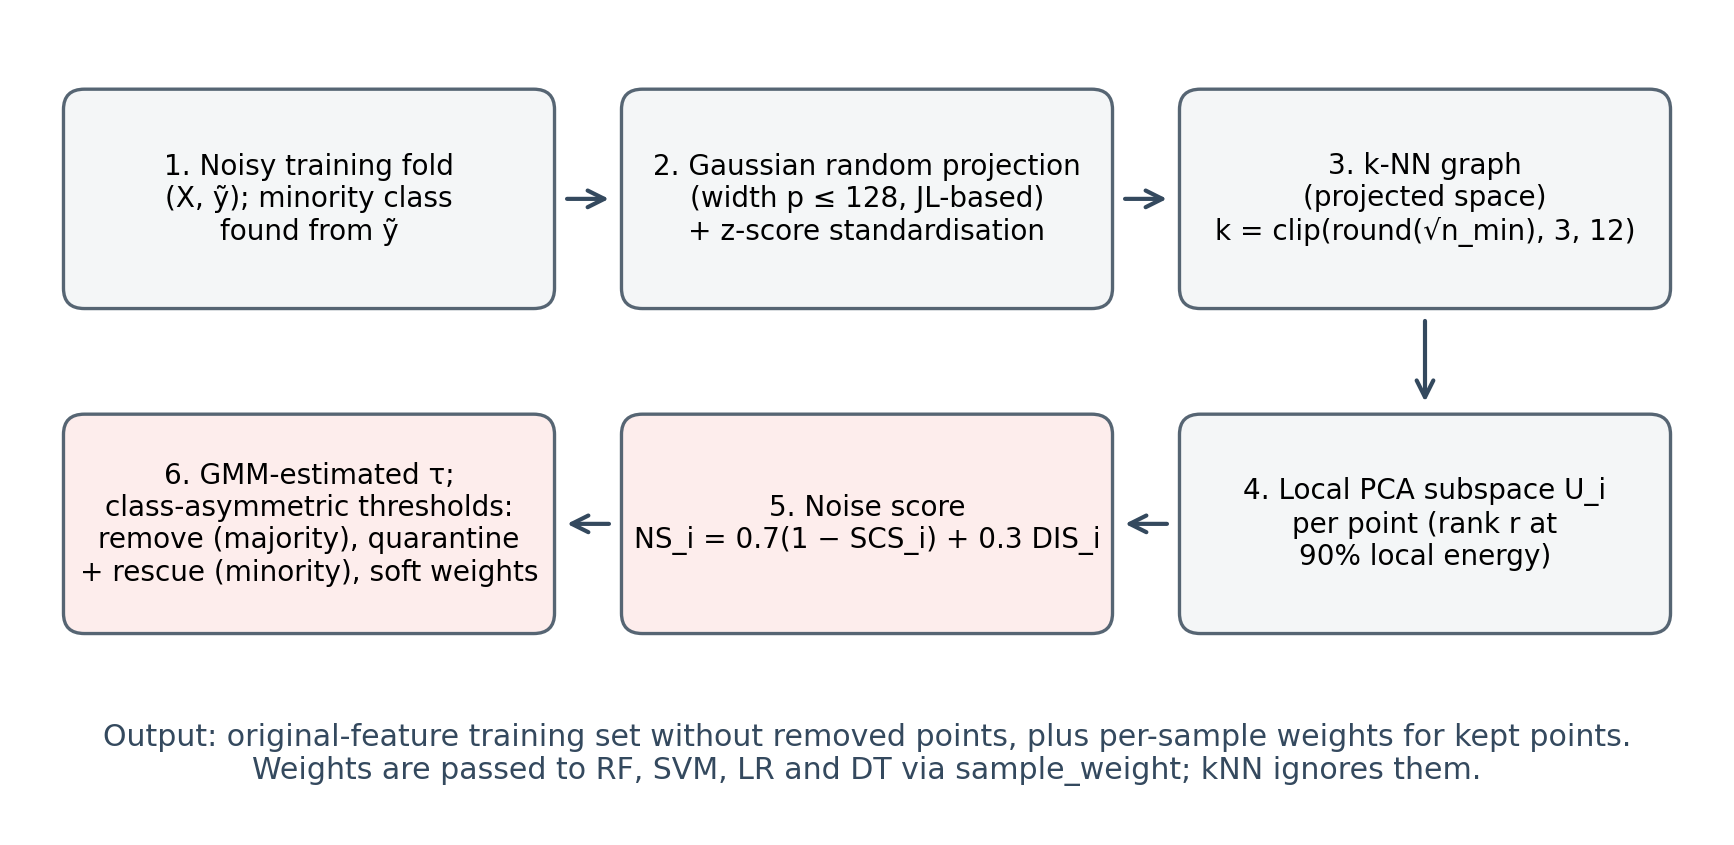
\includegraphics[width=\textwidth]{figures/fig1.png}
\caption{AMEND pipeline. Steps 1--4 build a local principal subspace for every training sample in a randomly projected, standardised space; step 5 scores samples; step 6 converts scores into removal (majority-labelled samples only), quarantine and soft weights. Shaded boxes contain the decision logic.}
\label{fig:1}
\end{figure*}

\subsection{Neighbourhood size and projection}\label{sec:neighbourhood-size-and-projection}

The neighbourhood size is tied to the size of the observed minority class:

\begin{equation}
k=\max\Bigl(2,\ \min\bigl(\operatorname{clip}(\operatorname{round}(\sqrt{n_{\min}}),\,3,\,12),\ n_{\min}-1\bigr)\Bigr)
\label{eq:1}
\end{equation}

If $n_{\mathrm{min}} <$ max(3, $k$ + 1), AMEND leaves the data unchanged; we call this a skip. The projection width is

\begin{equation}
\begin{gathered}
p=\min\Bigl(d,\ \max\bigl(32,\ \min(m_{\mathrm{JL}}(n,\varepsilon),\,128)\bigr)\Bigr),\\
m_{\mathrm{JL}}(n,\varepsilon)=\frac{4\ln n}{\varepsilon^{2}/2-\varepsilon^{3}/3},\qquad \varepsilon=0.5
\end{gathered}
\label{eq:2}
\end{equation}

where $m_{\mathrm{JL}}$ is the Johnson--Lindenstrauss dimension bound used by scikit-learn \cite{johnson1984,pedregosa2011}. If $d > p$, the data are mapped by a Gaussian random projection to min($p$, $n -$ 1) dimensions. For training folds of the sizes used here $m_{\mathrm{JL}}$ exceeds 128, so $p$ = min($d$, 128) = 128 for every dataset in this study (all have $d \ge $ 2000). The projection was therefore always applied, and its effective width min(128, $n -$ 1) was 128 for Carcinom, lung, lungCancer and Ovarian and between 39 and 101 for the other nine datasets. The projected features are then standardised to zero mean and unit variance, giving vectors $z_{i}$. Neighbourhoods $\mathcal{N}_{i}$ are the $k$ nearest samples to $z_{i}$ in Euclidean distance, excluding $i$ itself. Scores are computed in the projected space; removal and weights are applied to the original features.

\subsection{Local subspaces}\label{sec:local-subspaces}

For each sample, AMEND estimates a shrunk local covariance from its neighbours,

\begin{equation}
\begin{gathered}
C_i=\frac{1}{k-1}\sum_{j\in\mathcal{N}_i}(z_j-\bar{z}_i)(z_j-\bar{z}_i)^{\top},\\
\tilde{C}_i=(1-\gamma)\,C_i+\gamma\,\frac{\operatorname{tr}(C_i)}{p}\,I_p,\qquad \gamma=\min\Bigl(0.5,\ \frac{p}{k+p}\Bigr)
\end{gathered}
\label{eq:3}
\end{equation}

and takes $U_{i} \in  \mathbb{R}^{p\times r}$ as the eigenvectors of the $r$ largest eigenvalues of $\tilde{C}_{i}$. Because the shrinkage target is a multiple of the identity, $\tilde{C}_{i}$ has the same eigenvectors as $C_{i}$; the shrinkage improves numerical conditioning but does not change the estimated subspace. $C_{i}$ is built from $k \le $ 12 points and has rank at most $k -$ 1. The rank $r$ is chosen once per call from a probe set $\mathcal{P}$ of up to 60 samples drawn with a fixed seed:

\begin{equation}
\begin{gathered}
r=\operatorname*{median}_{i\in\mathcal{P}}\ \min\Bigl\{q:\ \frac{\sum_{l\le q}\sigma_{il}^{2}}{\sum_{l}\sigma_{il}^{2}}\ge 0.90\Bigr\},\\
r\leftarrow\operatorname{clip}\bigl(r,\,1,\,\min(p-1,\,k-1)\bigr)
\end{gathered}
\label{eq:4}
\end{equation}

where $\sigma _{il}$ are the singular values of the centred neighbour matrix of probe $i$. For $p >$ 80 and $r < p$/3 a partial symmetric eigensolver replaces the full decomposition.

\subsection{Noise score}\label{sec:noise-score}

Spectral coherence measures how well a sample's subspace aligns with those of its same-label neighbours:

\begin{equation}
\begin{gathered}
\mathrm{SCS}_i=\frac{1}{m_i\,r}\sum_{j\in\mathcal{N}_i^{+}}\bigl\|U_i^{\top}U_j\bigr\|_F^{2},\\
\mathcal{N}_i^{+}=\{j\in\mathcal{N}_i:\tilde{y}_j=\tilde{y}_i\},\quad m_i=|\mathcal{N}_i^{+}|\\
(\mathrm{SCS}_i=0\ \text{if}\ m_i=0)
\end{gathered}
\label{eq:5}
\end{equation}

SCS$_{i}$ lies in {[}0, 1{]}; it equals 1 when all same-label neighbours share the sample's subspace and 0 when their subspaces are orthogonal to it or when no neighbour shares its label. The implementation also provides an off-subspace energy term and a mixed base score,

\begin{equation}
\begin{gathered}
\mathrm{FNS}_i=\frac{\|z_i-U_iU_i^{\top}z_i\|^{2}}{\|z_i\|^{2}},\\
B_i=\alpha\,(1-\mathrm{SCS}_i)+(1-\alpha)\,\mathrm{FNS}_i
\end{gathered}
\label{eq:6}
\end{equation}

The final score adds neighbour-label disagreement with weight $w$:

\begin{equation}
\mathrm{DIS}_i=1-\frac{m_i}{k},\qquad \mathrm{NS}_i=(1-w)\,B_i+w\,\mathrm{DIS}_i
\label{eq:7}
\end{equation}

AMEND uses $\alpha $ = 1 (FNS disabled) and $w$ = 0.3, so NS$_{i}$ = 0.7(1 $-$ SCS$_{i}$) + 0.3 DIS$_{i}$. A sample with no same-label neighbour receives the maximum score NS$_{i}$ = 1.

\subsection{Flagging threshold}\label{sec:flagging-threshold}

If the scores are nearly constant (standard deviation below 0.015 or range below 0.05), AMEND takes no action. Otherwise a two-component Gaussian mixture with full covariance is fitted to the $n$ scores by expectation--maximisation \cite{dempster1977} with two initialisations, and $c_{\mathrm{hi}}$ denotes the component with the larger mean:

\begin{equation}
\begin{gathered}
\tau=\operatorname{clip}\Bigl(\frac{1}{n}\sum_{i=1}^{n}\mathbf{1}\bigl[P(c_{\mathrm{hi}}\mid\mathrm{NS}_i)>0.5\bigr],\ 0.02,\ \tau_{\max}\Bigr),\\
\tau_{\max}=0.5
\end{gathered}
\label{eq:8}
\end{equation}

If $n <$ 20, the scores have essentially zero variance, the fit fails, or the unclipped fraction is 0 or at least 0.95, a gap heuristic is used instead: the scores are sorted, the first gap in the top 30\% that exceeds three times the median gap marks the boundary, and $\tau $ is the fraction of scores above it (0.03 when no such gap exists and 0.05 when there are too few scores), clipped to {[}0.02, $\tau _{\mathrm{max}}${]}. $\tau $ is estimated once from the pooled scores of both classes.

\subsection{Class-asymmetric decisions and soft weights}\label{sec:class-asymmetric-decisions-and-soft-weights}

Hard and soft thresholds are quantiles $Q$ of the scores within each observed class; the minority class uses half the contamination of the majority class:

\begin{equation}
\begin{gathered}
h_M=Q_{1-\tau/2}(\mathrm{NS}_M),\qquad s_M=Q_{1-2\tau}(\mathrm{NS}_M),\\
h_m=Q_{1-\tau/4}(\mathrm{NS}_m),\qquad s_m=Q_{1-\tau}(\mathrm{NS}_m)
\end{gathered}
\label{eq:9}
\end{equation}

If a soft threshold is not below its hard threshold, it is reset to 0.8 times the hard threshold. Each sample then receives

\begin{equation}
\omega_i=\begin{cases}
\text{removed}, & i\in M \text{ and } \mathrm{NS}_i>h_M,\\
0.1\ (\text{quarantine}), & i\in m \text{ and } \mathrm{NS}_i>h_m,\\
\operatorname{clip}\Bigl(1-\dfrac{\mathrm{NS}_i-s_c}{h_c-s_c},0.1,1\Bigr), & \begin{array}{@{}l@{}}s_c<\mathrm{NS}_i\le h_c,\\ c\in\{M,m\},\end{array}\\
1, & \text{otherwise},
\end{cases}
\label{eq:10}
\end{equation}

In a binary task removal is therefore restricted to majority-labelled samples and to at most a fraction $\tau $/2 $\le $ 0.25 of them. Minority-labelled samples above their hard threshold are kept with weight 0.1.

\subsection{Anchored rescue}\label{sec:anchored-rescue}

If at least two minority samples are quarantined, each quarantined sample $q$ is compared with the anchor set $\mathcal{A}$ of minority samples that lie below both minority thresholds, and its weight is raised when it coheres with at least one anchor:

\begin{equation}
\omega_q\leftarrow 0.8\quad\text{if}\quad \max_{a\in\mathcal{A}}\ \frac{1}{r}\bigl\|U_q^{\top}U_a\bigr\|_F^{2}\ \ge\ 0.45
\label{eq:11}
\end{equation}

\subsection{Use by classifiers and computational cost}\label{sec:use-by-classifiers-and-computational-cost}

The retained samples, in their original features, are passed to the classifier together with their weights. Random forests, support vector machines, logistic regression and decision trees receive the weights through their sample\_weight argument; $k$-nearest-neighbour classification uses the retained samples without weights. The dominant costs are the neighbour search, one eigendecomposition of a $p \times  p$ matrix per sample (O($np^{3}$) with a dense solver) and the coherence computation (O($nkpr^{2}$)); the bases need O($npr$) memory. For fixed $k$ and $p$ the cost is linear in $n$, and capping $p$ at 128 bounds its dependence on $d$.

\begin{figure}[!t]
\footnotesize
\hrule height 0.8pt\vspace{3pt}
\noindent\textbf{Algorithm 1.} AMEND cleaning of one training fold
\vspace{3pt}\hrule\vspace{3pt}
\noindent\textbf{Input:} training features $X\in\mathbb{R}^{n\times d}$, observed labels $\tilde{y}$; settings of Table~\ref{tab:1}\\
\textbf{Output:} retained index set $S$; weights $\omega_S$
\begin{algorithmic}[1]
\STATE $m\leftarrow$ minority class of $\tilde{y}$; $n_{\min}\leftarrow|m|$; compute $k$ \eqref{eq:1}
\IF{$n_{\min}<\max(3,k+1)$} \RETURN all samples with $\omega=1$ \ENDIF
\STATE compute $p$ \eqref{eq:2}; \textbf{if} $d>p$ \textbf{then} $Z\leftarrow$ Gaussian random projection of $X$ \textbf{else} $Z\leftarrow X$
\STATE standardise the columns of $Z$; find $\mathcal{N}_i$, the $k$ nearest neighbours of each $z_i$
\STATE choose $r$ from probe neighbourhoods \eqref{eq:4}
\FORALL{$i$} \STATE $U_i\leftarrow$ top-$r$ eigenvectors of $\tilde{C}_i$ \eqref{eq:3} \ENDFOR
\FORALL{$i$} \STATE compute $\mathrm{SCS}_i$, $\mathrm{DIS}_i$ and $\mathrm{NS}_i$ (\eqref{eq:5}--\eqref{eq:7}) \ENDFOR
\IF{$\mathrm{std}(\mathrm{NS})<0.015$ \textbf{or} $\mathrm{range}(\mathrm{NS})<0.05$} \RETURN all samples with $\omega=1$ \ENDIF
\STATE $\tau\leftarrow$ Gaussian-mixture estimate \eqref{eq:8}, with gap-heuristic fallback
\STATE compute $h_M$, $s_M$, $h_m$, $s_m$ \eqref{eq:9}; assign weights and removal set $R$ \eqref{eq:10}
\STATE $Q\leftarrow$ quarantined minority samples; \textbf{if} $|Q|\ge 2$ \textbf{then} rescue by anchor coherence \eqref{eq:11}
\RETURN $S=\{1,\ldots,n\}\setminus R$ and $\omega_S$
\end{algorithmic}
\vspace{2pt}\hrule height 0.8pt
\end{figure}

\begin{table}[!t]
\centering
\footnotesize
\caption{AMEND settings used in all experiments}
\label{tab:1}
\setlength{\tabcolsep}{3.5pt}
\begin{tabular}{>{\raggedright\arraybackslash}p{0.2765\dimexpr\linewidth-4\tabcolsep\relax}>{\raggedright\arraybackslash}p{0.7235\dimexpr\linewidth-4\tabcolsep\relax}}
\hline
Component & Setting \\
\hline
Neighbourhood size $k$ & Automatic: clip(round($\sqrt{n_{\min}}$), 3, 12), at most $n_{\mathrm{min}} -$ 1 (1) \\
Local rank $r$ & Automatic: median 90\%-energy rank over $\le $ 60 probe neighbourhoods (4) \\
Projection width $p$ & Automatic: Johnson--Lindenstrauss bound with $\varepsilon $ = 0.5, between 32 and 128, at most $d$ (2) \\
Standardisation & z-score of projected features \\
Score terms & SCS only in the base score ($\alpha $ = 1, FNS disabled); label-disagreement weight $w$ = 0.3 \\
Threshold $\tau $ & Two-component Gaussian mixture, clipped to {[}0.02, 0.5{]}; gap-heuristic fallback \\
Decision rule & Class-asymmetric; minority contamination $\tau $/2; quarantine weight 0.1; soft-weight floor 0.1 \\
Rescue & Anchored; coherence threshold 0.45; rescued weight 0.8; requires $\ge $ 2 quarantined samples \\
Weights to classifiers & Yes (RF, SVM, LR, DT); kNN ignores weights \\
Random state & Experiment seed \\
\hline
\end{tabular}
\end{table}

\section{Experimental setup}\label{sec:experimental-setup}

\subsection{Datasets}\label{sec:datasets}

We used 13 binary datasets stored as CSV files (Table II). The label column was detected automatically; text-valued features were label-encoded, infinite values were treated as missing, and missing values were imputed with the median of the training fold. All 13 are small and high-dimensional. Sample sizes range from 50 (GLIOMA) to 253 (Ovarian), so training folds contain 40 to 202 samples; the number of features ranges from 2000 (colon) to 22 283 (burczynski), so $d$ exceeds $n$ by a factor of 16 to 175. Minority classes contain 7 (GLIOMA) to 91 (Ovarian) samples, and imbalance ratios range from 1.04 (Prostate) to 14.73 (Carcinom). The positive class for all test-set metrics is the minority class of the clean labels.

\begin{table}[!t]
\centering
\footnotesize
\caption{Datasets}
\label{tab:2}
\setlength{\tabcolsep}{3.5pt}
\begin{adjustbox}{max width=\linewidth}
\begin{tabular}{lcccccc}
\hline
Dataset & $n$ & $d$ & Minority & Majority & IR & Training fold \\
\hline
ALLAML & 72 & 7 129 & 25 & 47 & 1.88 & 57.6 \\
burczynski & 127 & 22 283 & 26 & 101 & 3.88 & 101.6 \\
Carcinom & 173 & 9 182 & 11 & 162 & 14.73 & 138.4 \\
CNS & 60 & 7 130 & 21 & 39 & 1.86 & 48.0 \\
colon & 62 & 2 000 & 22 & 40 & 1.82 & 49.6 \\
DLBCL & 77 & 7 130 & 19 & 58 & 3.05 & 61.6 \\
GLIOMA & 50 & 4 434 & 7 & 43 & 6.14 & 40.0 \\
leukemia & 72 & 7 070 & 25 & 47 & 1.88 & 57.6 \\
lung & 203 & 3 312 & 20 & 183 & 9.15 & 162.4 \\
lungCancer & 181 & 12 533 & 31 & 150 & 4.84 & 144.8 \\
Ovarian & 253 & 15 155 & 91 & 162 & 1.78 & 202.4 \\
Prostate & 102 & 2 136 & 50 & 52 & 1.04 & 81.6 \\
SRBCT & 83 & 2 308 & 11 & 72 & 6.55 & 66.4 \\
\hline
\end{tabular}
\end{adjustbox}
\par\vspace{3pt}
\begin{minipage}{\linewidth}\scriptsize $n$: samples; $d$: features after removal of the label column; IR: imbalance ratio (majority/minority). The last column is the mean size of the training fold in five-fold cross-validation.\end{minipage}
\end{table}

\subsection{Evaluation protocol}\label{sec:evaluation-protocol}

All experiments on real data follow a clean-then-classify protocol. For each dataset and each seed $s \in $ \{42, 7, 13, 21, 99, 123, 256, 512, 1024, 2024\}, stratified five-fold cross-validation with shuffling was run with random state $s$. In each fold the imputer was fitted on the training part, label noise was injected into the training labels only (random state 1000$s$ + fold), the cleaner was fitted to the noisy training fold, a classifier was trained on the cleaned data, and predictions were scored against the clean labels of the untouched test fold. Each configuration therefore has 50 train--test evaluations per dataset. The five classifiers, all from scikit-learn \cite{pedregosa2011} and seeded with $s$, were a random forest (RF; 200 trees, balanced class weights), an RBF support vector machine (SVM; $C$ = 1, balanced, standardised inputs), $k$-nearest neighbours (kNN; $k$ = 5, standardised inputs), logistic regression (LR; $C$ = 1, balanced, standardised inputs) and a decision tree (DT; balanced class weights).

\subsection{Noise models}\label{sec:noise-models}

With noise rate $\rho $, \emph{uniform} noise flips each training label independently with probability $\rho $; \emph{minority$\rightarrow $majority} noise flips each minority training label with probability $\rho $; \emph{majority$\rightarrow $minority} noise flips each majority training label with probability $\rho $. In the two class-conditional models $\rho $ is therefore a per-class rate. Under uniform and majority$\rightarrow $minority noise, flipped majority samples join the minority-labelled set, where AMEND can quarantine them but not remove them (Section III-F). With high imbalance these samples can dominate that set: in a Carcinom training fold (about 9 minority and 130 majority samples), 15\% uniform noise moves about 19 majority samples into the minority-labelled set while about 7.5 genuine minority samples keep their label, so roughly 72\% of the observed minority class is mislabelled.

Random flips ignore the tendency of real labelling errors to fall on ambiguous cases, so Experiment 10 adds two instance-dependent models. In each training fold a standardised, class-balanced logistic regression estimates, by stratified cross-validation with up to three folds inside the training fold, the out-of-fold probability of each sample's clean label; this model only defines the noise and is never seen by a cleaner or a classifier. \emph{Instance-dependent} noise flips the round($\rho n$) samples with the lowest such probability, in either class, so $\rho $ is a global rate. \emph{Minority instance-dependent} noise flips the round($\rho n_{\mathrm{min}}$) least confident minority samples and is the boundary-concentrated counterpart of minority$\rightarrow $majority noise. Ties are broken by a fixed-seed jitter. The class-conditional sweep used $\rho  \in $ \{0, 0.05, 0.10, 0.20, 0.30, 0.40\} and the instance-dependent sweep $\rho  \in $ \{0.05, 0.10, 0.20, 0.30\}. Experiments 1, 3, 5, 6 and 8 used uniform noise with $\rho $ = 0.15, and Experiments 7 and 9 used uniform noise at $\rho $ = 0.15 and minority$\rightarrow $majority noise at $\rho $ = 0.20.

\subsection{Compared methods}\label{sec:compared-methods}

\emph{No cleaning} trains on the noisy training fold. \emph{AUM} follows Pleiss \emph{et al.} \cite{pleiss2020} with gradient boosting (125 stages, depth 3): threshold samples (2\% of the training fold, at least five) are appended with a random wrong label, margins are averaged over boosting stages, and samples whose AUM falls below the 99th percentile of the threshold samples' AUM are removed; AUM skips when a class has fewer than five samples and keeps everything if fewer samples than the minority count would remain. \emph{ENN}, \emph{AllKNN} and \emph{IHT} are the imbalanced-learn implementations with default parameters \cite{lemaitre2017}; in that configuration all three edit only classes other than the minority, so in a binary task they prune the majority class alone, and IHT scores samples with its default estimator. \emph{CL} is confident learning \cite{northcutt2021confident} applied to out-of-fold predicted probabilities from a logistic regression; it estimates the joint distribution of observed and true labels and prunes accordingly. CL is the reference method in every comparison below. Experiment 9 repeats the comparison with each downstream classifier serving as CL's probability model (\emph{CL-matched}; the SVM is refitted with probability estimates enabled). For the threshold-free ranking analysis (Experiment 5) each method also supplies a continuous score: AMEND's NS; the negated AUM (AUM-score); the fraction of the five nearest neighbours, in the imputed original features, that carry a different label (kNN-disagree), which is the DIS term of (7) on its own, with a fixed $k$ = 5 and no projection, whereas AMEND computes DIS in the projected space with a data-driven $k$; one minus the out-of-fold probability of the observed label from a random forest (200 trees, balanced) under stratified cross-validation with min(5, $n_{\mathrm{min}}$) folds (IHT-score); and one minus confident learning's estimated probability of the observed label, from the same logistic-regression fit (CL).

Experiment 7 adds five controls, each built around the same AMEND fit so that one element changes at a time. \emph{RUS-matched} deletes, in each fold, exactly as many randomly chosen majority-labelled samples as AMEND deleted in that fold and passes no weights, so it differs from AMEND only in which majority samples go. \emph{RUS@0.083} deletes round(0.083$n$) random majority-labelled samples, 0.083 being AMEND's mean removal rate in Table V. \emph{Removal only} applies AMEND's removals and passes no weights. \emph{Weights only} removes nothing: samples AMEND would delete receive the quarantine weight 0.1 and all others keep AMEND's weights. \emph{Fully symmetric} applies one pooled threshold (hard quantile 1 $- \tau $/2, soft quantile 1 $-$ 2$\tau $), deletes samples above the hard threshold whatever their label, soft-weights samples between the two thresholds in both classes, and keeps at least two samples per class. The last variant is needed because the ``class-symmetric thresholds'' row of the ablation (Experiment 1) symmetrises the thresholds only; minority-labelled samples above them are still quarantined rather than deleted, so that row tests threshold asymmetry, not removal asymmetry. Experiment 8 varies the agree-weight $w$ of (7) over \{0, 0.1, 0.2, 0.3, 0.5, 0.7, 1\} with every other setting at its default. At $w$ = 0 the score is 1 $-$ SCS alone and at $w$ = 1 it is DIS alone, computed in the same projected, standardised space and with the same data-driven $k$, which removes both differences between NS and kNN-disagree noted above.

\subsection{Metrics}\label{sec:metrics}

\emph{Test-set metrics} treat the minority class as positive: recall, precision, F1, G-mean (the square root of recall times specificity), false-positive rate (FPR) and ROC-AUC computed from predicted probabilities or decision values. \emph{Detection metrics} compare the removal set with the injected flips on the training fold: noise precision (share of removed samples that were flipped), noise recall (share of flips removed), noise F1, false-removal rate (FRR; share of clean samples removed), removal rate and skip rate. For AMEND we also report flag recall and flag precision, which additionally count retained samples with weight $\omega  \le $ 0.5 as flagged. \emph{Ranking metrics} score a continuous noise score against the flip indicator: ROC-AUC, average precision (AP) and LiftAP, the AP divided by the flip rate. \emph{Internal-state metrics} (Experiment 11) record, per fold, the realised $k$ and $r$, whether $r$ reached its cap $k -$ 1, the working projection width, $\tau $, the removal rate, the shares of retained samples with $\omega $ = 1 and with $\omega  \le $ 0.5, and the effective imbalance ratio: the sum of $\omega $ over majority-labelled samples divided by the sum over minority-labelled samples, with removed samples at weight 0, computed on the observed labels before and after cleaning. Detection and ranking metrics measure how well a cleaner finds wrong labels in the training fold; test-set metrics measure the classifier trained on its output. We report the two separately throughout because, as Section V shows, they need not agree. The test-set FPR is reported for Experiment 3 only, because in the stored outputs of Experiments 1, 2 and 7 to 10 the FPR field was overwritten by the detection false-removal rate; FRR is reported for those experiments instead.

\subsection{Statistical analysis}\label{sec:statistical-analysis}

Each dataset contributes the mean over its 50 folds. Methods were compared across datasets with the Friedman test \cite{friedman1937} using the Iman--Davenport $F$ statistic \cite{iman1980}, with the Nemenyi critical difference at $\alpha $ = 0.05 \cite{demsar2006,nemenyi1963}. AMEND was compared with each other method by two-sided Wilcoxon signed-rank tests \cite{wilcoxon1945} with Holm correction \cite{holm1979} within each classifier--metric family (pairs with fewer than five non-zero differences are not tested), and effect sizes were computed with Cliff's $\delta $ \cite{cliff1993}. With 13 datasets the smallest attainable two-sided exact Wilcoxon $p$ is 0.0002. Experiments 7, 9 and 10 use the same procedure with AMEND as the reference; Experiment 8 compares the seven values of $w$ on dataset-level means over the five classifiers, with the default $w$ = 0.3 as the reference. For the noise sweep we tested AMEND against no cleaning on dataset-level means over the five classifiers, with Holm correction across the 15 combinations of noise model and non-zero noise rate for each metric, and Experiment 10 was analysed the same way across its eight combinations. These classifier-averaged tests, the tests on detection metrics in Experiment 7 and the comparison of $w$ = 0.7 with $w$ = 1 were run on the saved results after the experiments. The trend test in the minority-size sweep is exploratory. We describe a finding as \emph{statistically supported} when its Holm-adjusted $p$ is below 0.05 and as an \emph{observation} otherwise.

\subsection{Experiments}\label{sec:experiments}

Experiment 1 is an ablation that varies one AMEND factor at a time around the default setting (15\% uniform noise, five classifiers). Experiment 2 is the noise sweep over three noise models and six rates. Experiment 3 is the comparison with the five cleaners (AUM, ENN, AllKNN, IHT and CL) and the no-cleaning control. Experiments 1--3 use all five classifiers under the protocol of Section IV-B. Experiment 4 measures runtime on synthetic data: each class is generated on its own random five-dimensional linear subspace of $\mathbb{R}^{d}$ with isotropic Gaussian noise (standard deviation 0.1), and the minority class (30\% of samples) is offset by 3.0 in every coordinate, with $n \in $ \{200, 500, 1000, 2000, 4000\} at $d$ = 50 and $d \in $ \{20, 50, 100, 300, 1000\} at $n$ = 1000; each time is the median of three runs with seed 42. This synthetic design probes scaling in $n$ and $d$ only: it is milder in imbalance and narrower in features than the datasets of Table II, so its absolute timings are not comparable with those of Section V-L. Experiment 5 evaluates threshold-free noise rankings. Experiment 6 subsamples the minority class of each dataset to \{5, 8, 12, 16, 20, 30, 45\} samples (where available) before cross-validation and measures the ranking ROC-AUC of AMEND and of CL.

Experiments 7 to 11 were run afterwards with the same protocol, seeds and folds; their AMEND and no-cleaning results reproduce those of Experiment 3 exactly. Experiment 7 compares AMEND with the five controls of Section IV-D and with no cleaning, and Experiment 8 is the agree-weight sweep; both use all five classifiers. Experiment 9 compares AMEND with CL and CL-matched. Experiment 10 applies the two instance-dependent noise models to AMEND, CL and no cleaning. Experiment 11 fits AMEND alone, trains no classifier, and records its internal state on clean data, at 15\% uniform noise and at 20\% minority$\rightarrow $majority and majority$\rightarrow $minority noise. Experiments ran on a Google Colab virtual machine with two virtual CPUs (Intel Xeon, 2.20 GHz) and 12 GiB of memory under Linux 6.6, using Python 3.13.15, NumPy 2.1.3, SciPy 1.16.3, pandas 2.2.3, scikit-learn 1.6.1 and imbalanced-learn 0.14.2.

\section{Results and analysis}\label{sec:results-and-analysis}

\subsection{Comparison with existing cleaners at 15\% uniform noise}\label{sec:comparison-with-existing-cleaners-at-15-uniform-noise}

Table III reports test-set results for the seven methods. CL had the highest mean F1 (0.654) and the highest ROC-AUC (0.844); AMEND was second on F1 (0.624, against 0.611 for no cleaning) and had the highest mean G-mean (0.707). Neither average describes any single classifier well (Fig. 2a). With random forests AMEND was the best of the seven methods on both F1 (0.666) and G-mean, with the best average rank (2.23 of 7; Iman--Davenport $p$ = 0.007); its F1 gains over no cleaning (+0.085) and AUM (+0.108) survived Holm correction, its G-mean gain over CL (+0.068, Holm $p$ = 0.010) was significant, and its F1 margin over CL (+0.045) was not (Holm $p$ = 0.086). With SVM, kNN and LR no F1 difference from no cleaning or from CL reached significance. With decision trees CL was clearly better than AMEND (F1 +0.117, Holm $p$ = 0.028; ROC-AUC +0.063, Holm $p$ = 0.021). Table IV summarises these tests. Effect sizes are small to moderate. With random forests Cliff's $\delta $ for AMEND against no cleaning was 0.24 on F1 and 0.30 on G-mean, and against CL 0.10 and 0.15; CL's advantage with decision trees corresponded to $\delta $ = $-$0.40 on F1 and $-$0.42 on ROC-AUC.

\begin{table*}[!t]
\centering
\footnotesize
\caption{Test-set performance at 15\% uniform training-label noise}
\label{tab:3}
\setlength{\tabcolsep}{3.5pt}
\begin{adjustbox}{max width=\linewidth}
\begin{tabular}{lccccccccccc}
\hline
& \multicolumn{5}{c}{F1 by classifier} & \multicolumn{6}{c}{Mean over classifiers} \\
Method & RF & SVM & kNN & LR & DT & Recall & Prec. & F1 & G-mean & FPR & AUC \\
\hline
AMEND & \textbf{0.666} & 0.617 & 0.617 & 0.672 & 0.550 & 0.724 & 0.605 & 0.624 & \textbf{0.707} & 0.195 & 0.819 \\
CL & 0.621 & 0.609 & \textbf{0.641} & \textbf{0.731} & \textbf{0.667} & 0.677 & \textbf{0.692} & \textbf{0.654} & 0.703 & \textbf{0.119} & \textbf{0.844} \\
No cleaning & 0.582 & \textbf{0.628} & 0.619 & 0.673 & 0.551 & 0.655 & 0.634 & 0.611 & 0.690 & 0.135 & 0.826 \\
AUM & 0.559 & 0.618 & 0.607 & 0.668 & 0.546 & 0.639 & 0.628 & 0.599 & 0.675 & 0.133 & 0.823 \\
ENN & 0.599 & 0.562 & 0.550 & 0.558 & 0.494 & \textbf{0.869} & 0.441 & 0.553 & 0.618 & 0.435 & 0.789 \\
AllKNN & 0.579 & 0.537 & 0.542 & 0.534 & 0.503 & 0.864 & 0.437 & 0.539 & 0.635 & 0.435 & 0.785 \\
IHT & 0.555 & 0.494 & 0.561 & 0.543 & 0.529 & 0.844 & 0.438 & 0.536 & 0.701 & 0.365 & 0.801 \\
\hline
\end{tabular}
\end{adjustbox}
\par\vspace{3pt}
\begin{minipage}{\linewidth}\scriptsize The first block gives F1 per classifier; the second averages each metric over the five classifiers. Values are means over 13 datasets, each the mean of 50 folds. Bold marks the best value in each column (lowest for FPR).\end{minipage}
\end{table*}

Against the neighbourhood and hardness editors the picture is uniformly favourable. AMEND's F1 was significantly higher than ENN, AllKNN and IHT for LR, its ROC-AUC significantly higher than at least one of the three for every classifier, and its FPR significantly lower than all three for all five classifiers. Those editors obtained the highest recall of any method (0.844 to 0.869) by removing a third or more of the training fold, at FPRs of 0.365 to 0.435 --- a trade that inflates recall without improving F1 (0.536 to 0.553, the three lowest values in the table).

The costs of AMEND are consistent across classifiers. Its FPR (0.195) was significantly higher than that of no cleaning (0.135), CL (0.119) and AUM (0.133) for every one of the five classifiers. Fig. 2b places the methods in the recall--FPR plane: AMEND gains recall over no cleaning (0.724 against 0.655) and loses precision (0.605 against 0.634), whereas CL improves both (0.677 and 0.692). AMEND's mean F1 advantage over no cleaning is thus a recall gain concentrated in random forests, while CL's advantage is broader.

\begin{figure*}[!t]
\centering
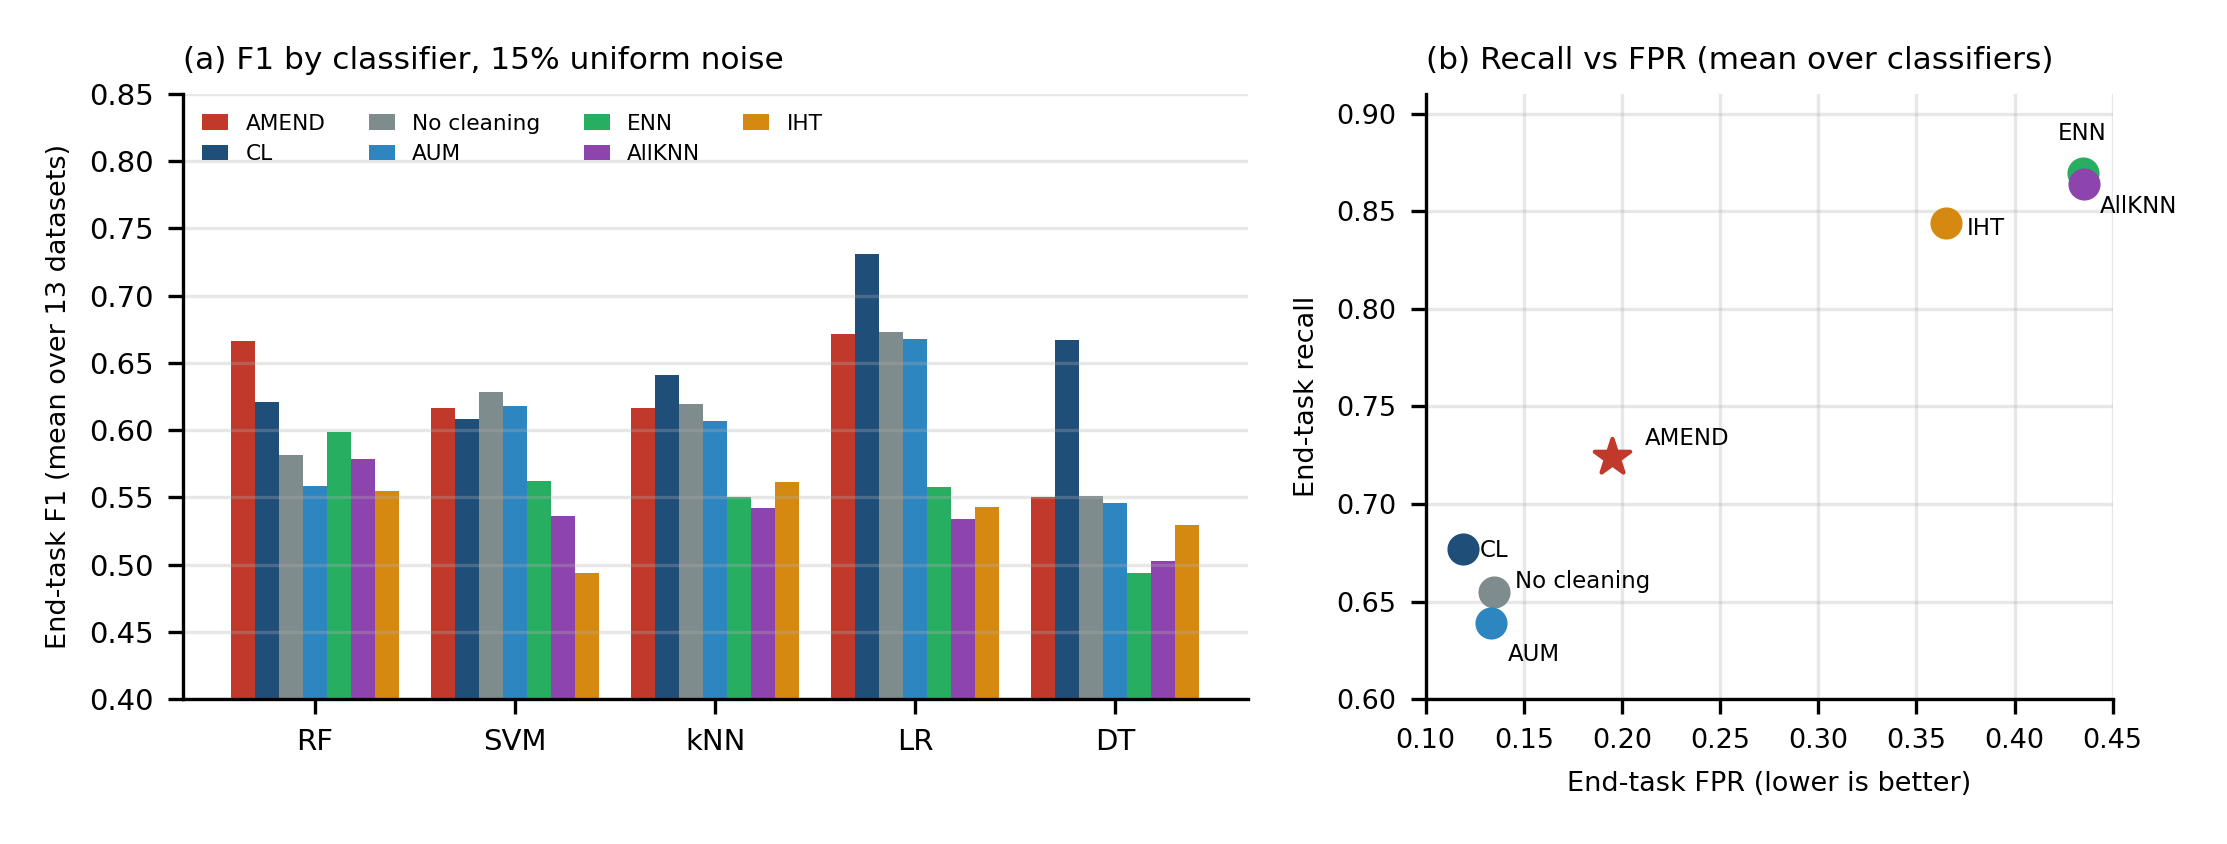
\includegraphics[width=\textwidth]{figures/fig2.png}
\caption{Test-set results at 15\% uniform noise. (a) F1 per classifier, mean over 13 datasets. (b) Recall against FPR, mean over datasets and classifiers.}
\label{fig:2}
\end{figure*}

\begin{table*}[!t]
\centering
\footnotesize
\caption{Statistical comparison at 15\% uniform noise}
\label{tab:4}
\setlength{\tabcolsep}{3.5pt}
\begin{adjustbox}{max width=\linewidth}
\begin{tabular}{lccccccc}
\hline
Clf. & Metric & $F_{\mathrm{F}}$ ($p$) & AMEND rank & $\Delta $ vs none ($p_{\mathrm{Holm}}$) & $\Delta $ vs CL ($p_{\mathrm{Holm}}$) & Significantly better than & Significantly worse than \\
\hline
RF & F1 & 3.23 (0.007) & 2.23 (1/7) & +0.085 (0.007) & +0.045 (0.086) & AUM, none & -- \\
& G-mean & 7.77 ($<$0.001) & 2.08 (1/7) & +0.105 (0.001) & +0.068 (0.010) & AUM, AllKNN, CL, ENN, none & -- \\
& AUC & 13.25 ($<$0.001) & 3.38 (4/7) & $-$0.007 (0.181) & $-$0.002 (0.542) & IHT & -- \\
& FPR & 48.76 ($<$0.001) & 3.77 (4/7) & +0.047 (0.007) & +0.035 (0.008) & AllKNN, ENN, IHT & AUM, CL, none \\
SVM & F1 & 1.83 (0.104) & 3.69 (3/7) & $-$0.011 (0.671) & +0.008 (0.946) & -- & -- \\
& G-mean & 4.39 ($<$0.001) & 4.35 (4/7) & $-$0.049 (0.015) & +0.009 (1.000) & -- & none \\
& AUC & 13.53 ($<$0.001) & 3.23 (3/7) & $-$0.014 (0.467) & $-$0.020 (0.103) & AllKNN, ENN & -- \\
& FPR & 55.88 ($<$0.001) & 4.15 (4/7) & +0.137 (0.001) & +0.138 (0.001) & AllKNN, ENN, IHT & AUM, CL, none \\
kNN & F1 & 1.90 (0.092) & 3.38 (3/7) & $-$0.002 (1.000) & $-$0.024 (0.916) & -- & -- \\
& G-mean & 6.36 ($<$0.001) & 2.92 (3/7) & +0.012 (0.098) & +0.013 (1.000) & AUM, AllKNN, ENN & -- \\
& AUC & 9.57 ($<$0.001) & 3.77 (4/7) & $-$0.006 (0.820) & $-$0.024 (0.031) & AllKNN & CL \\
& FPR & 56.91 ($<$0.001) & 4.00 (4/7) & +0.041 (0.001) & +0.053 (0.001) & AllKNN, ENN, IHT & AUM, CL, none \\
LR & F1 & 5.18 ($<$0.001) & 3.27 (2/7) & $-$0.001 (1.000) & $-$0.059 (0.064) & AllKNN, ENN, IHT & -- \\
& G-mean & 4.03 (0.002) & 3.08 (2/7) & +0.009 (0.204) & $-$0.015 (0.204) & AllKNN & -- \\
& AUC & 9.87 ($<$0.001) & 3.00 (2/7) & $-$0.001 (1.000) & $-$0.016 (0.144) & AllKNN, IHT & -- \\
& FPR & 42.47 ($<$0.001) & 3.85 (4/7) & +0.037 (0.001) & +0.045 (0.040) & AllKNN, ENN, IHT & AUM, CL, none \\
DT & F1 & 4.79 ($<$0.001) & 3.77 (4/7) & $-$0.001 (1.000) & $-$0.117 (0.028) & -- & CL \\
& G-mean & 5.18 ($<$0.001) & 3.46 (2/7) & +0.006 (1.000) & $-$0.057 (0.081) & -- & -- \\
& AUC & 6.30 ($<$0.001) & 3.65 (2/7) & $-$0.002 (1.000) & $-$0.063 (0.021) & AllKNN, ENN & CL \\
& FPR & 40.19 ($<$0.001) & 3.69 (4/7) & +0.039 (0.002) & +0.108 (0.002) & AllKNN, ENN, IHT & AUM, CL, none \\
\hline
\end{tabular}
\end{adjustbox}
\par\vspace{3pt}
\begin{minipage}{\linewidth}\scriptsize $F_{\mathrm{F}}$ ($p$): Iman--Davenport statistic and $p$-value over seven methods. Rank: AMEND's average Friedman rank and its position (lower is better; FPR ranked ascending). $\Delta $ columns: mean AMEND minus comparator with Holm-adjusted Wilcoxon $p$. The last two columns list all methods that AMEND beat or lost to at Holm-adjusted $p <$ 0.05 (`none' = the no-cleaning control). Nemenyi critical difference = 2.50.\end{minipage}
\end{table*}

\subsection{Noise detection}\label{sec:noise-detection}

On the detection task CL is clearly the more accurate method (Table V). At $\rho $ = 0.15 it removed 25.7\% of the training fold, 52.0\% of its removals were genuinely flipped samples and it caught 74.1\% of all flips; AMEND removed 8.3\%, of which 17.9\% were flipped, catching 8.7\% of flips. Both gaps are significant (precision $-$0.341 and recall $-$0.654, Holm $p \le $ 0.001), as is the difference in noise F1 ($-$0.487). The Friedman test rejects equality on all four detection metrics ($p <$ 0.001).

The compensating result is collateral damage. AMEND's false-removal rate --- the share of correctly labelled samples it discarded --- was 0.083, significantly lower than CL (0.172, Holm $p$ = 0.002), IHT (0.360), AllKNN (0.404) and ENN (0.411), all at Holm $p \le $ 0.001; only AUM was more cautious (0.033), and AUM caught fewer flips than AMEND (recall $-$0.027, Holm $p$ = 0.017). AMEND's removals were also significantly more precise than those of ENN, AllKNN and IHT (+0.054 to +0.081, Holm $p \le $ 0.012). Fig. 3 shows the resulting ordering: AMEND occupies the cautious corner of the recall--FRR plane with AUM, CL sits high on both axes, and the three editors are costly on both. As a reference point, removals drawn at random from the majority-labelled samples, the only ones AMEND removes, would have expected precision $\rho n_{m}$/((1 $- \rho $)$n_{M}$ + $\rho n_{m}$) under uniform noise, where $n_{m}$ and $n_{M}$ are the clean class sizes. With the class sizes of Table II this chance level ranges from 0.012 (Carcinom) to 0.145 (Prostate), mean 0.062; AMEND exceeded it on 12 of 13 datasets, median ratio 3.5 (Wilcoxon $p <$ 0.001, a single post-hoc test), the exception being Prostate, the most balanced dataset.

If quarantined and low-weight retained samples are counted as flags, AMEND flagged 26.0\% of the training fold with flag recall 0.412 and flag F1 0.319. The hard-removal baselines produce no equivalent quantity, so this is not a like-for-like comparison; it does indicate that a large part of what AMEND identifies is down-weighted rather than deleted. AMEND never skipped a fold on these datasets (skip rate 0.000). Whether this detection deficit carries over to the end task depends on the noise model; Sections V-D and V-F test that link directly.

\begin{table*}[!t]
\centering
\footnotesize
\caption{Noise detection at 15\% uniform noise (mean over 13 datasets; average Friedman rank in parentheses, lower is better)}
\label{tab:5}
\setlength{\tabcolsep}{3.5pt}
\begin{adjustbox}{max width=\linewidth}
\begin{tabular}{lcccccc}
\hline
Method & Noise precision & Noise recall & Noise F1 & FRR & Removal rate & Time (s) \\
\hline
AMEND & 0.179 (3.08) & 0.087 (5.23) & 0.106 (4.38) & 0.083 (2.23) & 0.083 & 0.225 \\
CL & 0.520 (1.31) & 0.741 (1.08) & 0.593 (1.08) & 0.172 (3.23) & 0.257 & 1.624 \\
AUM & 0.233 (2.62) & 0.059 (5.77) & 0.086 (4.69) & 0.033 (1.00) & 0.036 & 45.950 \\
ENN & 0.099 (5.00) & 0.246 (3.12) & 0.137 (3.54) & 0.411 (5.08) & 0.384 & 0.015 \\
AllKNN & 0.104 (4.69) & 0.237 (2.81) & 0.138 (3.54) & 0.404 (5.00) & 0.377 & 0.032 \\
IHT & 0.125 (4.31) & 0.196 (3.00) & 0.135 (3.77) & 0.360 (4.46) & 0.335 & 2.223 \\
\hline
\end{tabular}
\end{adjustbox}
\par\vspace{3pt}
\begin{minipage}{\linewidth}\scriptsize Friedman/Iman--Davenport over six cleaners: noise precision $F_{\mathrm{F}}$ = 16.35, noise recall $F_{\mathrm{F}}$ = 68.57, noise F1 $F_{\mathrm{F}}$ = 10.46, FRR $F_{\mathrm{F}}$ = 41.77, all $p <$ 0.001, critical difference 2.09. Time is the mean cleaning time per training fold.\end{minipage}
\end{table*}

\begin{figure}[!t]
\centering
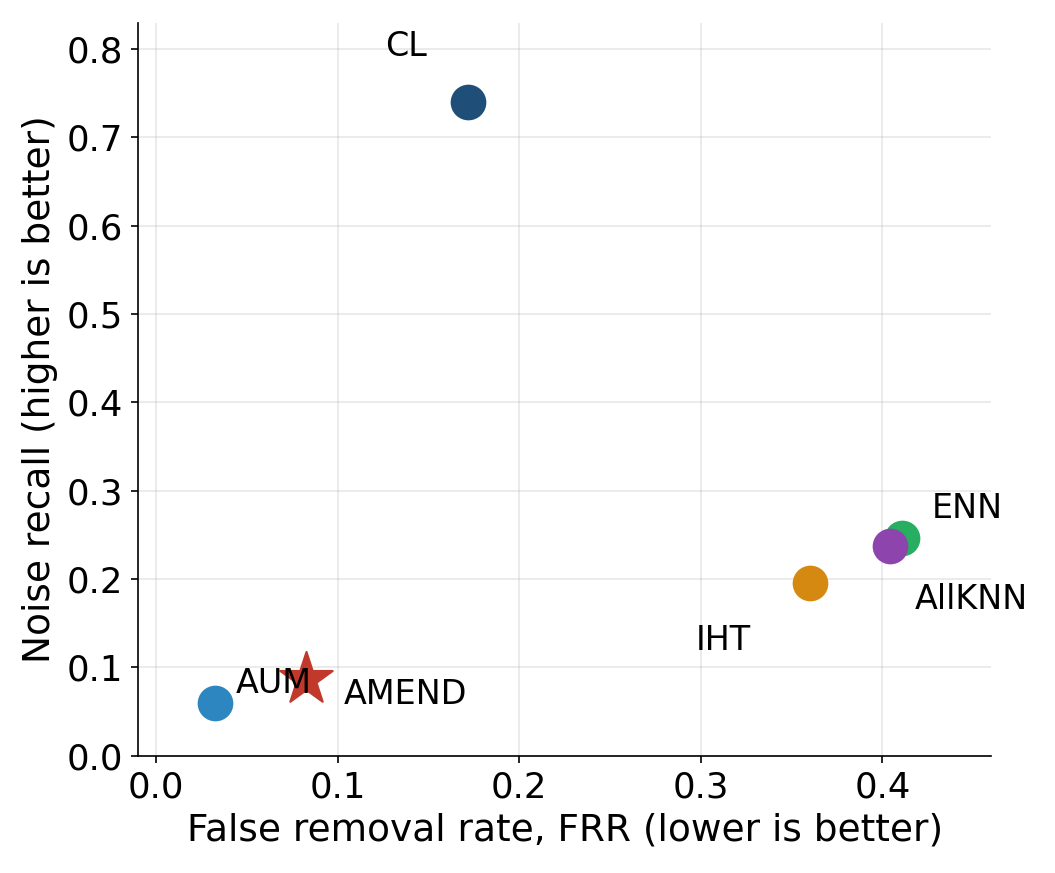
\includegraphics[width=\columnwidth]{figures/fig3.png}
\caption{Share of injected flips removed against share of correctly labelled samples removed, at 15\% uniform noise (mean over 13 datasets).}
\label{fig:3}
\end{figure}

\subsection{Behaviour across noise models and rates}\label{sec:behaviour-across-noise-models-and-rates}

Table VI and Fig. 4 compare AMEND with no cleaning and with CL across the sweep. Under \textbf{minority$\rightarrow $majority} noise --- the regime AMEND is designed for --- the gains over no cleaning are statistically supported at every non-zero rate, rising from +0.023 at $\rho $ = 0.05 to +0.059 at $\rho $ = 0.30 and 0.40, with 12 or 13 of the 13 datasets improving (Holm $p$ between 0.004 and 0.027); the G-mean gains are supported for $\rho  \ge $ 0.10. Against CL, AMEND's mean F1 was higher at all five rates, by +0.012 at $\rho $ = 0.05 rising to +0.037 at $\rho $ = 0.40, but no such difference survived Holm correction (smallest adjusted $p$ = 0.574) and the per-dataset record is mixed (6/7 wins at $\rho $ = 0.05, 10/3 at $\rho $ = 0.40). The honest reading is that AMEND matches CL in this regime and beats no cleaning; a claim that it beats CL is not supported by these data. As an observation, the gain over no cleaning at $\rho $ = 0.20 was present for all five classifiers but varied widely in size: +0.139 for RF, +0.047 for kNN, +0.041 for LR, +0.040 for DT and +0.008 for SVM.

Under \textbf{uniform} noise no comparison was significant in either direction: AMEND was between $-$0.004 and +0.010 F1 from no cleaning, and between $-$0.045 and $-$0.011 from CL, the largest shortfall occurring at $\rho $ = 0.20. Under \textbf{majority$\rightarrow $minority} noise AMEND fell below no cleaning at every non-zero rate ($-$0.006 to $-$0.055), supported at $\rho $ = 0.30 (12 of 13 datasets worse, Holm $p$ = 0.046), and below CL by up to 0.094, also supported at $\rho $ = 0.30 (Holm $p$ = 0.026). With no injected noise, AMEND differed from no cleaning by +0.006 F1 ($p$ = 0.946) and $-$0.009 ROC-AUC (unadjusted $p$ = 0.048).

\begin{table*}[!t]
\centering
\footnotesize
\caption{AMEND against no cleaning and against CL across noise models and rates}
\label{tab:6}
\setlength{\tabcolsep}{3.5pt}
\begin{adjustbox}{max width=\linewidth}
\begin{tabular}{lcccccccccc}
\hline
&  &  & \multicolumn{3}{c}{vs no cleaning} & \multicolumn{3}{c}{vs CL (F1)} & \multicolumn{2}{c}{vs CL (G-mean)} \\
Noise model & $\rho $ & F1 AMEND & $\Delta $F1 & W/L & $p_{\mathrm{Holm}}$ & $\Delta $F1 & W/L & $p_{\mathrm{Holm}}$ & $\Delta $G-mean & $p_{\mathrm{Holm}}$ \\
\hline
Minority$\rightarrow $majority & 0.05 & 0.723 & +0.023 & 12/1 & 0.015 & +0.012 & 6/7 & 1.000 & +0.013 & 1.000 \\
& 0.10 & 0.688 & +0.038 & 13/0 & 0.004 & +0.016 & 7/6 & 1.000 & +0.016 & 1.000 \\
& 0.20 & 0.619 & +0.055 & 13/0 & 0.004 & +0.018 & 8/5 & 1.000 & +0.019 & 1.000 \\
& 0.30 & 0.549 & +0.059 & 12/1 & 0.006 & +0.033 & 10/3 & 0.574 & +0.034 & 0.557 \\
& 0.40 & 0.445 & +0.059 & 12/1 & 0.027 & +0.037 & 10/3 & 0.574 & +0.041 & 0.399 \\
Uniform & 0.05 & 0.709 & +0.008 & 9/4 & 1.000 & $-$0.011 & 4/9 & 1.000 & +0.006 & 1.000 \\
& 0.10 & 0.663 & +0.010 & 9/4 & 0.879 & $-$0.025 & 4/9 & 1.000 & +0.002 & 1.000 \\
& 0.20 & 0.573 & +0.009 & 10/3 & 0.562 & $-$0.045 & 4/9 & 0.989 & $-$0.007 & 1.000 \\
& 0.30 & 0.459 & +0.001 & 9/4 & 1.000 & $-$0.041 & 6/7 & 1.000 & $-$0.014 & 1.000 \\
& 0.40 & 0.371 & $-$0.004 & 7/6 & 1.000 & $-$0.017 & 7/6 & 1.000 & $-$0.019 & 1.000 \\
Majority$\rightarrow $minority & 0.05 & 0.722 & $-$0.006 & 6/7 & 1.000 & $-$0.016 & 3/10 & 1.000 & +0.010 & 1.000 \\
& 0.10 & 0.696 & $-$0.013 & 5/8 & 0.879 & $-$0.034 & 3/10 & 0.574 & +0.004 & 1.000 \\
& 0.20 & 0.635 & $-$0.037 & 3/10 & 0.121 & $-$0.069 & 2/11 & 0.188 & $-$0.015 & 1.000 \\
& 0.30 & 0.559 & $-$0.055 & 1/12 & 0.046 & $-$0.094 & 1/12 & 0.026 & $-$0.049 & 0.746 \\
& 0.40 & 0.522 & $-$0.024 & 3/10 & 0.383 & $-$0.042 & 3/10 & 0.188 & $-$0.015 & 1.000 \\
\hline
\end{tabular}
\end{adjustbox}
\par\vspace{3pt}
\begin{minipage}{\linewidth}\scriptsize F1 values are dataset-level means over the five classifiers, averaged over 13 datasets. W/L: datasets on which AMEND was better/worse. $p_{\mathrm{Holm}}$: Wilcoxon signed-rank $p$, Holm-adjusted across the 15 model--rate combinations within each metric and comparator.\end{minipage}
\end{table*}

The removal behaviour (Fig. 4d--f) accounts for much of this pattern and exposes the sharpest design difference between the two methods. CL's removal rate tracks the injected noise: under uniform noise it rises from 14.6\% at $\rho $ = 0.05 to 46.0\% at $\rho $ = 0.40. AMEND's does not: it removed 12.0\% of samples at $\rho $ = 0 (per-dataset range 6.0\% to 22.8\%) and between 7.6\% and 11.6\% at every non-zero rate and noise model. What changes with $\rho $ is only the composition of its removals. Under uniform noise its removal precision rose from 0.074 to 0.297 while recall fell from 0.099 to 0.070. Under minority$\rightarrow $majority noise, where every flip carries the majority label and is therefore eligible for removal, recall was 0.32 to 0.45 and precision 0.08 to 0.32. Under majority$\rightarrow $minority noise the flips carry the minority label and cannot be removed at all, and removal precision was 0.004 and 0.013 at $\rho $ = 0.05 and 0.10; AMEND did quarantine or down-weight many of them (flag recall 0.54 and 0.46, flag precision 0.14 and 0.21), but the end-task result was still worse than no cleaning. CL removed 10.1\% at $\rho $ = 0 (up to 50.4\% on one dataset), so neither method is inert on clean data.

\begin{figure*}[!t]
\centering
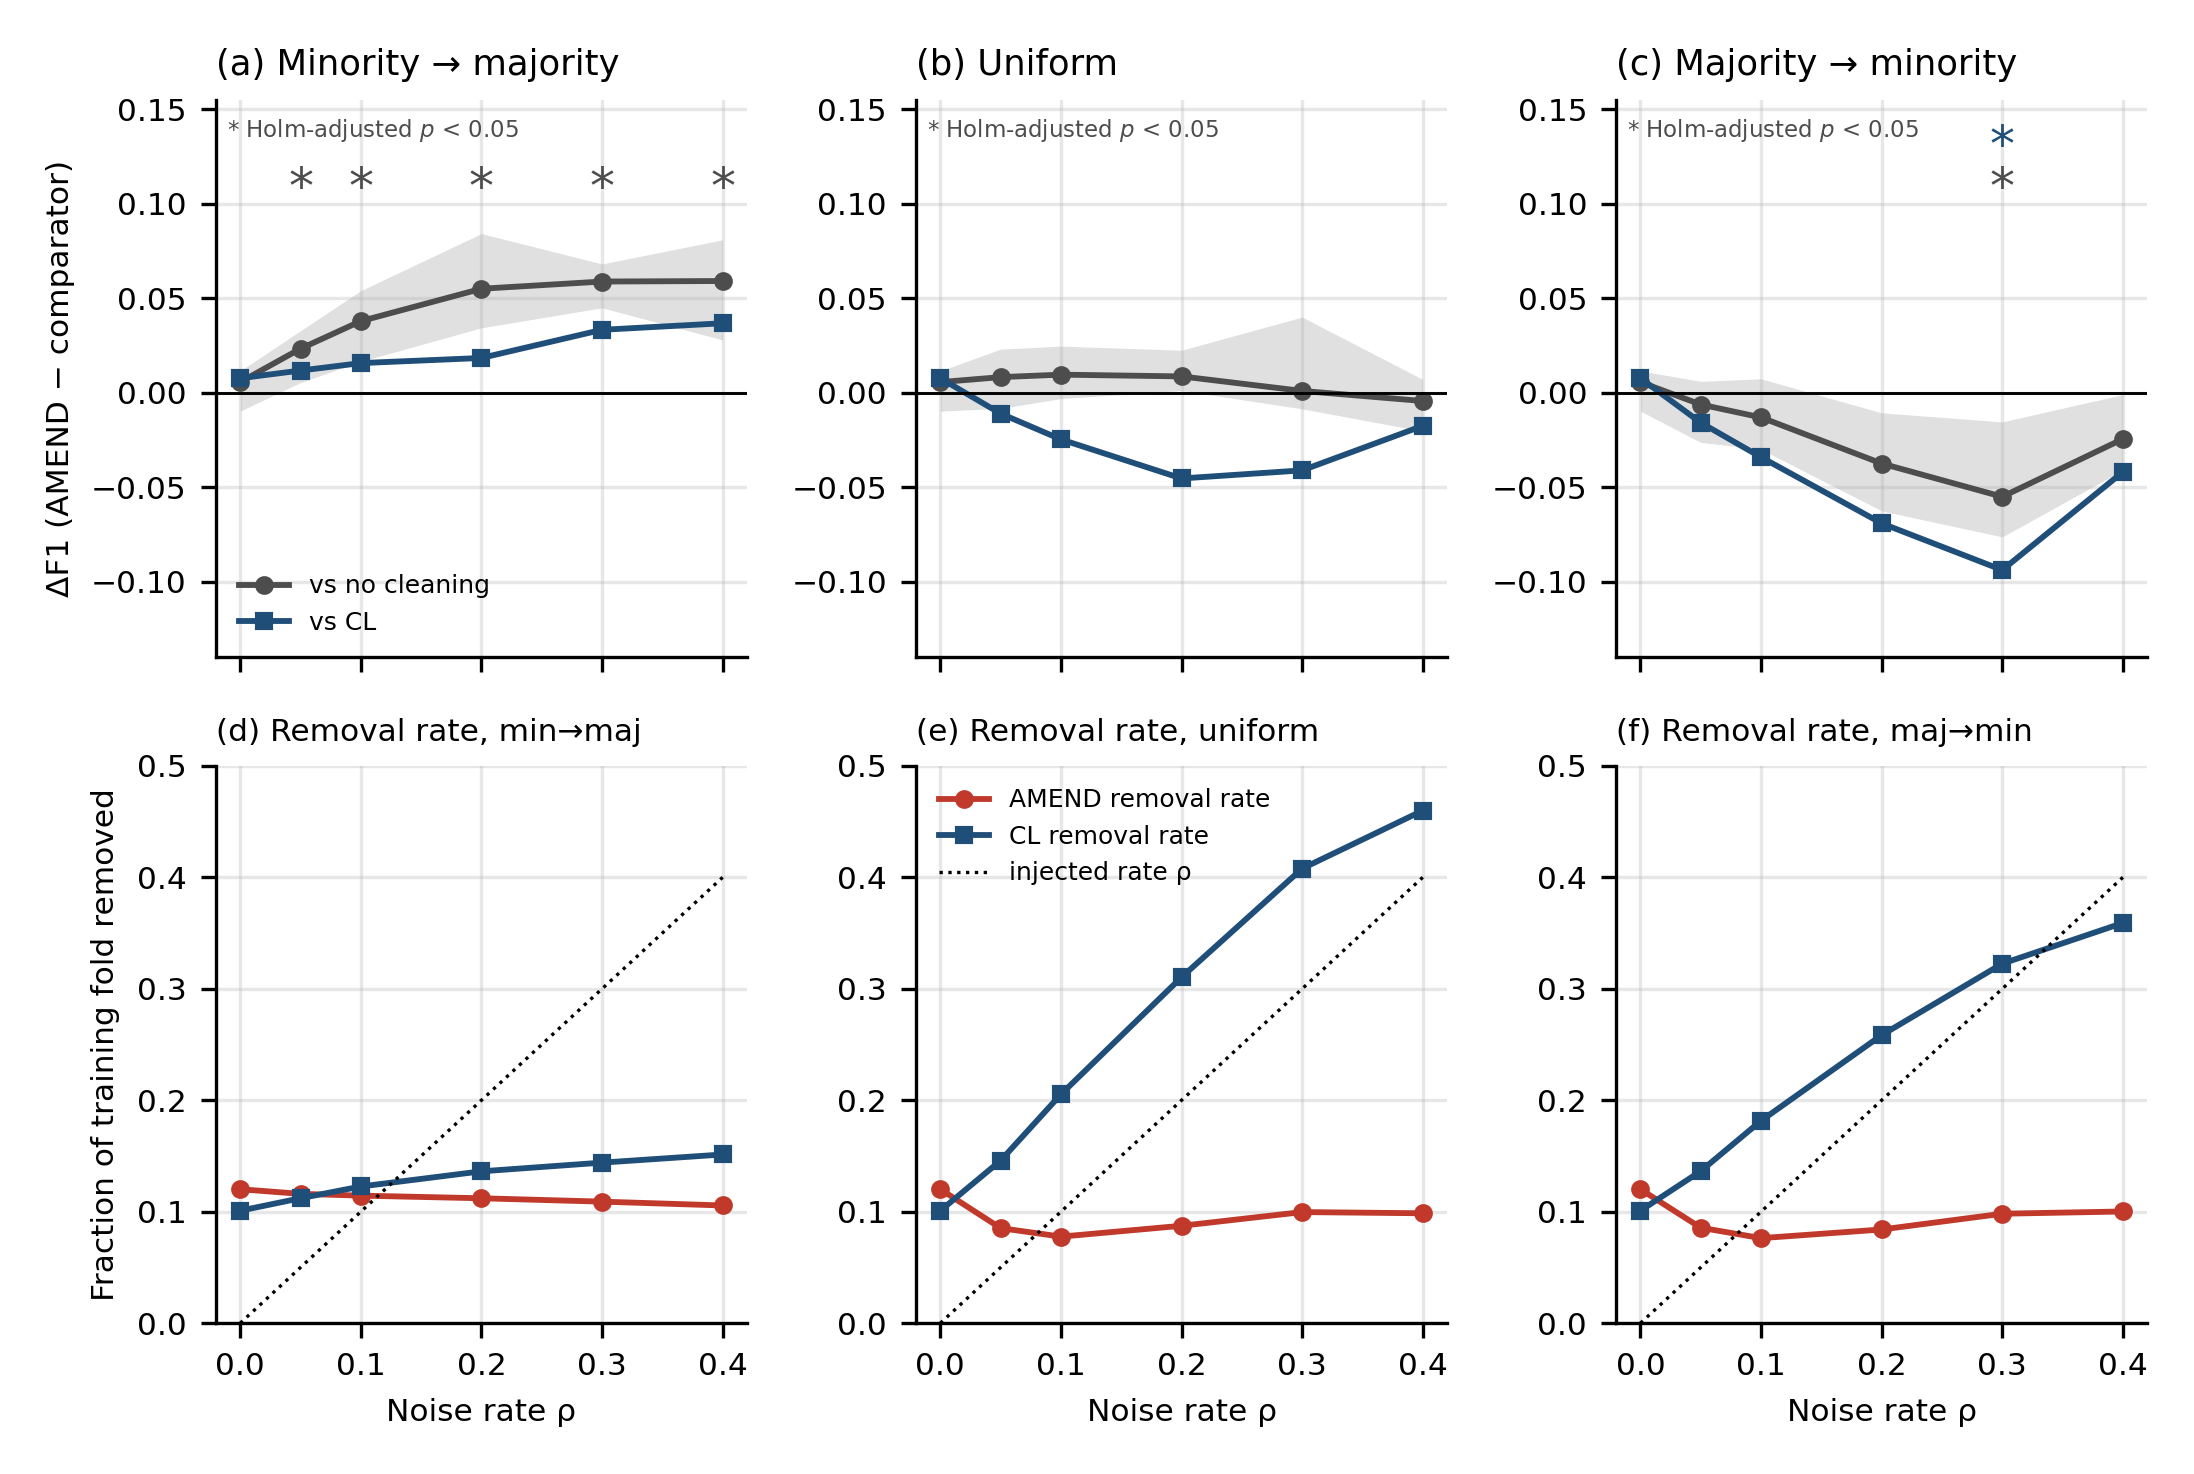
\includegraphics[width=\textwidth]{figures/fig4.png}
\caption{Noise sweep. (a--c) Difference in F1 between AMEND and each comparator (dataset-level means over classifiers, averaged over 13 datasets); the shaded band is the interquartile range over datasets for the comparison with no cleaning; asterisks mark Holm-adjusted $p <$ 0.05. (d--f) Fraction of the training fold removed by AMEND and CL; the value at $\rho $ = 0 is computed from retained sample counts, and the dotted line marks the injected rate.}
\label{fig:4}
\end{figure*}

\subsection{Instance-dependent noise}\label{sec:instance-dependent-noise}

Table VII and Fig. 5 report Experiment 10. Flipping the least confident samples is highly damaging: with no cleaning, F1 fell from 0.651 at $\rho $ = 0.05 to 0.380 at $\rho $ = 0.30 under instance-dependent noise. AMEND improved on no cleaning in all eight combinations of model and rate, by +0.011 to +0.046 F1 with 8 to 12 of the 13 datasets improving, and the gain was statistically supported at $\rho $ = 0.10 and 0.20 under instance-dependent noise (Holm $p$ = 0.015 and 0.004) and at $\rho $ = 0.20 and 0.30 under minority instance-dependent noise (Holm $p$ = 0.005 and 0.015). Against CL the two models separate. When the least confident samples of either class are flipped, AMEND and CL were indistinguishable, within 0.007 F1 at every rate (Holm $p$ = 1.000). When only minority samples are flipped, AMEND led CL at every rate and the lead grew with $\rho $, from +0.012 at $\rho $ = 0.05 to +0.036 at $\rho $ = 0.30 (11 of 13 datasets; Holm $p$ = 0.020). At $\rho $ = 0.20 the F1 lead of +0.026 narrowly missed significance (Holm $p$ = 0.056), while the G-mean lead of the same size did not (Holm $p$ = 0.024); at $\rho $ = 0.30 the G-mean lead was +0.035 (Holm $p$ = 0.020).

\begin{table*}[!t]
\centering
\footnotesize
\caption{AMEND, CL and no cleaning under instance-dependent noise (Experiment 10)}
\label{tab:7}
\setlength{\tabcolsep}{3.5pt}
\begin{adjustbox}{max width=\linewidth}
\begin{tabular}{lccccccccc}
\hline
&  & \multicolumn{3}{c}{F1} & AMEND $-$ no cleaning & AMEND $-$ CL & Noise precision & Noise recall & Ranking \\
Noise model & $\rho $ & None & CL & AMEND & $\Delta $F1 (W/L; $p_{\mathrm{Holm}}$) & $\Delta $F1 (W/L; $p_{\mathrm{Holm}}$) & AMEND/CL & AMEND/CL & ROC-AUC \\
\hline
Instance-dependent & 0.05 & 0.651 & 0.672 & 0.674 & +0.023 (10/3; 0.106) & +0.002 (5/8; 1.000) & 0.122/0.369 & 0.191/0.292 & 0.644 \\
& 0.10 & 0.557 & 0.588 & 0.587 & \textbf{+0.030 (11/2; 0.015)} & $-$0.001 (7/6; 1.000) & 0.231/0.523 & 0.161/0.362 & 0.665 \\
& 0.20 & 0.431 & 0.455 & 0.461 & \textbf{+0.030 (12/1; 0.004)} & +0.006 (8/5; 1.000) & 0.322/0.676 & 0.121/0.447 & 0.687 \\
& 0.30 & 0.380 & 0.407 & 0.408 & +0.027 (9/4; 0.106) & 0.000 (8/5; 1.000) & 0.347/0.692 & 0.098/0.496 & 0.682 \\
Minority instance-dependent & 0.05 & 0.718 & 0.717 & 0.729 & +0.011 (8/5; 0.273) & +0.012 (7/6; 1.000) & 0.026/0.021 & 0.202/0.081 & 0.522 \\
& 0.10 & 0.680 & 0.685 & 0.702 & +0.022 (9/4; 0.106) & +0.017 (7/6; 1.000) & 0.065/0.144 & 0.338/0.184 & 0.589 \\
& 0.20 & 0.623 & 0.628 & 0.654 & \textbf{+0.031 (12/1; 0.005)} & +0.026 (10/3; 0.056) & 0.144/0.283 & 0.373/0.214 & 0.604 \\
& 0.30 & 0.537 & 0.548 & 0.583 & \textbf{+0.046 (11/2; 0.015)} & \textbf{+0.036 (11/2; 0.020)} & 0.222/0.372 & 0.360/0.244 & 0.593 \\
\hline
\end{tabular}
\end{adjustbox}
\par\vspace{3pt}
\begin{minipage}{\linewidth}\scriptsize F1 values are dataset-level means over the five classifiers, averaged over 13 datasets. $\Delta $F1: AMEND minus the comparator, with W/L the datasets on which AMEND was better/worse and the Wilcoxon $p$ Holm-adjusted across the eight model--rate combinations (post-hoc); bold marks Holm-adjusted $p <$ 0.05. Noise precision and recall refer to removed samples; the ranking ROC-AUC is that of AMEND's score NS against the injected flips.\end{minipage}
\end{table*}

Per classifier, the pattern of the random-noise experiments repeats. Random forests gained over no cleaning in all eight conditions (Holm $p \le $ 0.021) and over CL in seven (Holm $p \le $ 0.048), and kNN gained over no cleaning in four conditions and over CL in one; no SVM, logistic-regression or decision-tree comparison with either reference was significant. ROC-AUC did not improve. AMEND was below no cleaning on average at all eight conditions, by at most 0.009 and never significantly, and below CL at all eight, significantly only at $\rho $ = 0.30 under instance-dependent noise ($-$0.028; higher on 1 of 13 datasets; Holm $p$ = 0.020).

The detection figures in Table VII again point in a different direction from the end task. Under instance-dependent noise CL's removals were two to three times as precise as AMEND's (0.369 to 0.692 against 0.122 to 0.347) and caught more of the flips (0.292 to 0.496 against 0.098 to 0.191), and AMEND's ranking ROC-AUC fell to 0.644 to 0.687, below its 0.757 under uniform noise; the two methods nonetheless reached the same F1. Under minority instance-dependent noise AMEND's ranking was barely above chance (0.522 to 0.604) and its removals were less precise than CL's at three of four rates, but it caught more of the flips (0.202 to 0.373 against 0.081 to 0.244), because every flip carries the majority label and AMEND directs all of its removals there. AMEND removed 8.2\% to 12.6\% of the training fold in every condition, CL between 9.0\% and 24.2\%.

\begin{figure*}[!t]
\centering
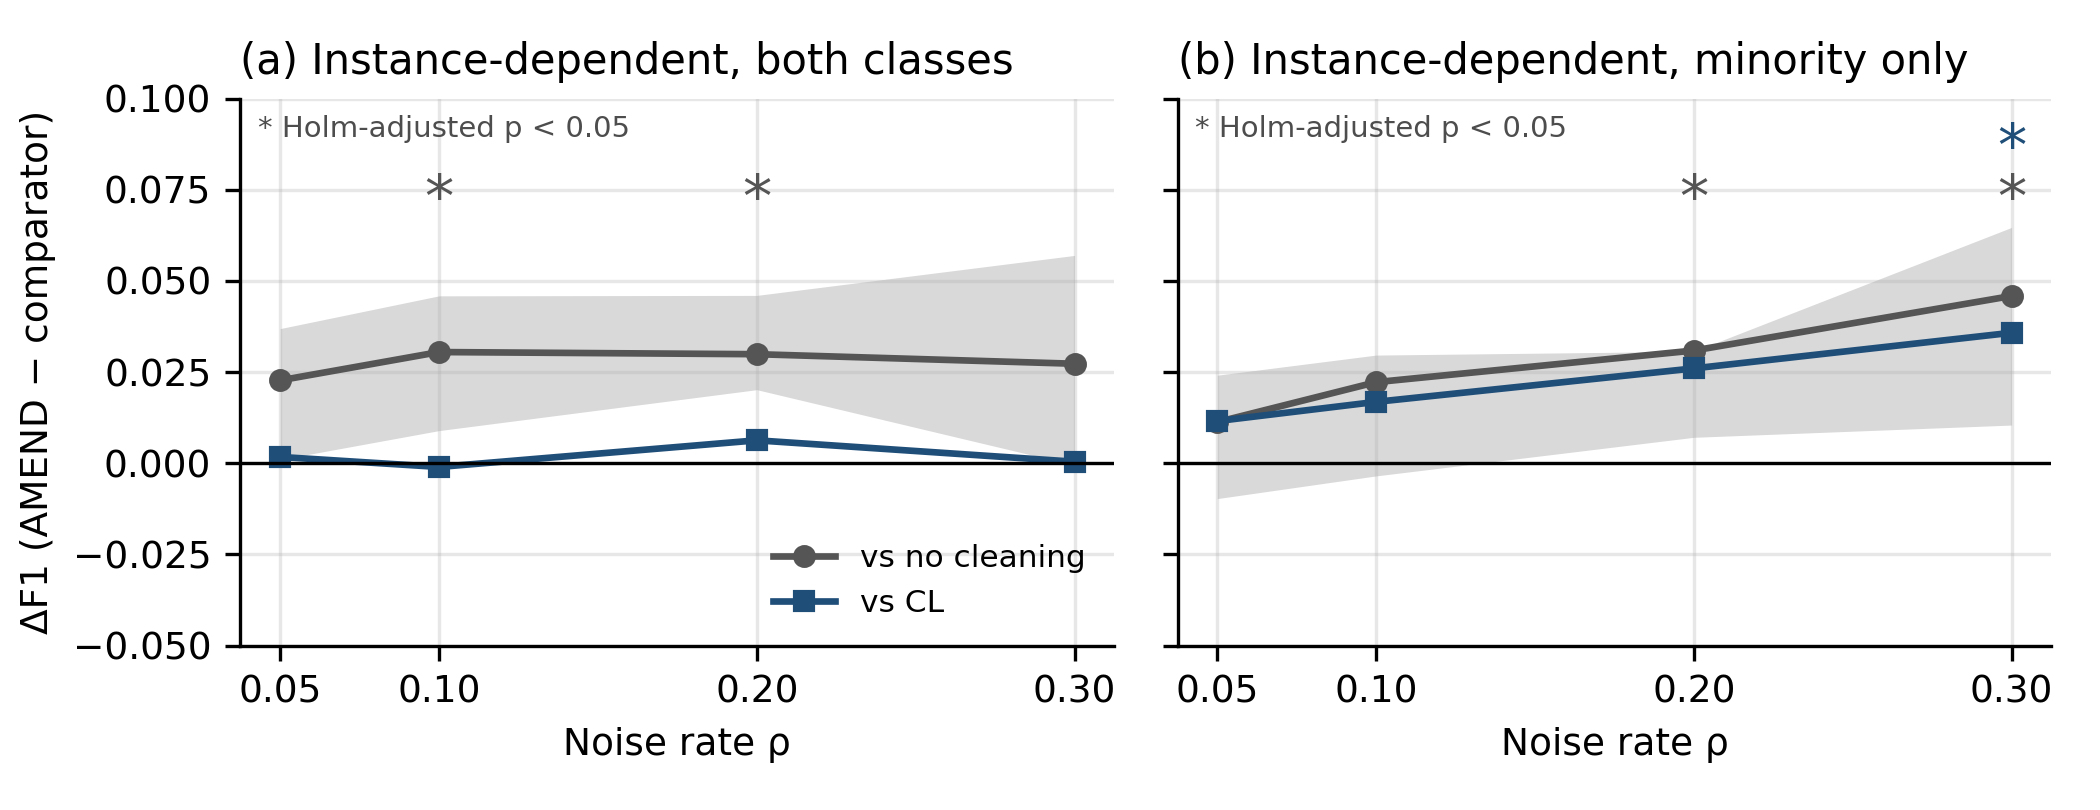
\includegraphics[width=\textwidth]{figures/fig5.png}
\caption{Instance-dependent noise (Experiment 10). Difference in F1 between AMEND and each comparator (dataset-level means over the five classifiers, averaged over 13 datasets) when the least confident samples of (a) either class or (b) the minority class only are flipped. The shaded band is the interquartile range over datasets for the comparison with no cleaning; asterisks mark Holm-adjusted $p <$ 0.05 across the eight model--rate combinations.}
\label{fig:5}
\end{figure*}

\subsection{Confident learning with a matched base model}\label{sec:confident-learning-with-a-matched-base-model}

The CL results above use logistic-regression probabilities for every downstream classifier. Experiment 9 gives CL the same model the end task uses (Table VIII), and the matched version was not stronger. Under uniform noise at $\rho $ = 0.15 its mean F1 was 0.633 against 0.654 for the logistic-regression version; it removed more of the training fold (27.3\% against 25.7\%) with lower noise precision (0.453 against 0.520), and it was worse with decision trees (0.613 against 0.667), SVMs (0.570 against 0.609) and kNN (0.611 against 0.641), better only with random forests (0.640 against 0.621). Under minority$\rightarrow $majority noise at $\rho $ = 0.20 the two versions differed by 0.005 in mean F1 (0.606 and 0.601).

\begin{table*}[!t]
\centering
\footnotesize
\caption{Confident learning with a logistic-regression base and with a matched base model (Experiment 9)}
\label{tab:8}
\setlength{\tabcolsep}{3.5pt}
\begin{adjustbox}{max width=\linewidth}
\begin{tabular}{lccccccccccc}
\hline
Condition & Method & RF & SVM & kNN & LR & DT & Mean F1 & Mean AUC & Noise prec. & Noise rec. & Removal \\
\hline
Uniform, $\rho $ = 0.15 & AMEND & \textbf{0.666} & 0.617 & 0.617 & 0.672 & 0.550 & 0.624 & 0.819 & 0.179 & 0.087 & 0.083 \\
& CL (LR base) & 0.621 & 0.609 & \textbf{0.641} & \textbf{0.731} & \textbf{0.667} & \textbf{0.654} & 0.844 & 0.520 & 0.741 & 0.257 \\
& CL-matched & 0.640 & 0.570 & 0.611 & \textbf{0.731} & 0.613 & 0.633 & 0.822 & 0.453 & 0.666 & 0.273 \\
& No cleaning & 0.582 & \textbf{0.628} & 0.619 & 0.673 & 0.551 & 0.611 & 0.826 & -- & -- & -- \\
Min$\rightarrow $maj, $\rho $ = 0.20 & AMEND & \textbf{0.543} & \textbf{0.534} & \textbf{0.590} & \textbf{0.731} & 0.698 & \textbf{0.619} & 0.858 & 0.238 & 0.425 & 0.112 \\
& CL (LR base) & 0.505 & 0.505 & 0.563 & 0.717 & \textbf{0.714} & 0.601 & 0.861 & 0.494 & 0.621 & 0.136 \\
& CL-matched & 0.531 & 0.531 & 0.564 & 0.717 & 0.687 & 0.606 & 0.856 & 0.455 & 0.575 & 0.131 \\
& No cleaning & 0.404 & 0.526 & 0.543 & 0.690 & 0.658 & 0.564 & 0.861 & -- & -- & -- \\
\hline
\end{tabular}
\end{adjustbox}
\par\vspace{3pt}
\begin{minipage}{\linewidth}\scriptsize F1 per classifier and means over classifiers and 13 datasets; bold marks the best value in each column within a condition. For CL-matched each classifier is paired with CL fitted on that classifier, so its LR column equals CL; its detection columns average the five base models. Average Friedman ranks of AMEND among the four methods on F1 (lower is better): uniform RF 1.77 ($p_{\mathrm{F}}$ = 0.007), SVM 2.54, kNN 2.54, LR 3.08, DT 3.00; minority$\rightarrow $majority RF 1.62 ($p_{\mathrm{F}} <$ 0.001), SVM 2.31, kNN 1.69, LR 2.31, DT 2.35.\end{minipage}
\end{table*}

Against CL-matched, AMEND's per-classifier F1 differences ranged from $-$0.063 to +0.047 under uniform noise and from +0.003 to +0.026 under minority$\rightarrow $majority noise, and none survived Holm correction. Against the logistic-regression version AMEND was better with random forests in both conditions (+0.045, Holm $p$ = 0.043; +0.038, Holm $p$ = 0.027) and worse with decision trees under uniform noise ($-$0.117, Holm $p$ = 0.014). The uniform random-forest comparison was not significant in the seven-method family of Table IV (Holm $p$ = 0.086); the difference lies only in the size of the Holm family. The concern that a single, weak base model understates CL is not borne out: logistic-regression probabilities were the better choice for CL on these data, so the comparisons in Sections V-A to V-D use CL's stronger version.

\subsection{Noise removal or rebalancing? Controls}\label{sec:noise-removal-or-rebalancing-controls}

AMEND deletes only majority-labelled samples and passes weights to four of the five classifiers, so part of any gain could come from shifting the class balance rather than from removing wrong labels. Tables IX and X and Fig. 6 separate the two. The decisive control is RUS-matched, which deletes as many majority-labelled samples as AMEND in each fold but chooses them at random. Its removals had close to chance-level precision (0.060 under uniform and 0.075 under minority$\rightarrow $majority noise), whereas AMEND's were three times as precise (0.179 and 0.238) and caught more of the flips (0.087 against 0.033, and 0.425 against 0.124). Both differences held on 11 or more of the 13 datasets in each condition (post-hoc Wilcoxon $p \le $ 0.002).

\begin{table*}[!t]
\centering
\footnotesize
\caption{Controls: end-task and detection performance (Experiment 7)}
\label{tab:9}
\setlength{\tabcolsep}{3.5pt}
\begin{adjustbox}{max width=\linewidth}
\begin{tabular}{lcccccccccc}
\hline
&  &  & \multicolumn{4}{c}{Uniform, $\rho $ = 0.15} & \multicolumn{4}{c}{Minority$\rightarrow $majority, $\rho $ = 0.20} \\
Method & Removes & Weights & F1 & G-mean & Noise prec. & Noise rec. & F1 & G-mean & Noise prec. & Noise rec. \\
\hline
No cleaning & -- & -- & 0.611 & 0.690 & -- & -- & 0.564 & 0.603 & -- & -- \\
AMEND & Majority & Yes & 0.624 & 0.707 & 0.179 & 0.087 & 0.619 & 0.654 & \textbf{0.238} & \textbf{0.425} \\
Removal only & Majority & No & \textbf{0.626} & \textbf{0.715} & 0.179 & 0.087 & \textbf{0.629} & \textbf{0.666} & \textbf{0.238} & \textbf{0.425} \\
Weights only & Nothing & Yes & 0.612 & 0.683 & -- & -- & 0.574 & 0.607 & -- & -- \\
Fully symmetric & Both & Yes & 0.581 & 0.641 & \textbf{0.376} & \textbf{0.299} & 0.463 & 0.499 & 0.094 & 0.297 \\
RUS-matched & Majority, random & No & 0.621 & 0.705 & 0.060 & 0.033 & 0.592 & 0.628 & 0.075 & 0.124 \\
RUS@0.083 & Majority, random & No & 0.618 & 0.703 & 0.056 & 0.030 & 0.589 & 0.626 & 0.072 & 0.090 \\
\hline
\end{tabular}
\end{adjustbox}
\par\vspace{3pt}
\begin{minipage}{\linewidth}\scriptsize Means over 13 datasets (and over five classifiers for F1 and G-mean). Removes: which samples can be deleted; Weights: whether weights are passed to the classifier. AMEND, removal only and RUS-matched remove identical numbers of samples in every fold (8.3\% and 11.2\% of the training fold in the two conditions); RUS@0.083 removes 8.2\% and the fully symmetric variant 11.0\% and 12.8\%. Bold marks the best value in each column. Test-set FPR is not available for this experiment (Section IV-E).\end{minipage}
\end{table*}

Under uniform noise that better selection did not yield a better classifier. Mean F1 was 0.624 for AMEND and 0.621 for RUS-matched, and no per-classifier F1 difference between them survived Holm correction; the largest, +0.037 with random forests, had Holm $p$ = 0.172. On G-mean the two methods split: AMEND was ahead with random forests (+0.050, Holm $p$ = 0.038) and behind with SVMs ($-$0.055, Holm $p$ = 0.007). At this noise level AMEND's end-task effect cannot be distinguished from that of random majority undersampling of the same size. The random-forest gain over no cleaning reported in Section V-A (+0.085 F1) is largely rebalancing: RUS-matched alone recovered 0.047 of it, and the remaining 0.037 is not significant.

Under minority$\rightarrow $majority noise, where every flip carries the majority label and is eligible for removal, AMEND's selection did matter. Its F1 exceeded that of RUS-matched with random forests (+0.079, Holm $p$ = 0.004), logistic regression (+0.026, Holm $p$ = 0.007) and kNN (+0.022, Holm $p$ = 0.003); the differences for decision trees (+0.030) and SVMs ($-$0.019) were not significant. Mean F1 was 0.619 for AMEND, 0.592 for RUS-matched and 0.564 for no cleaning, so about half of AMEND's gain over no cleaning in this regime is attributable to rebalancing and about half to the choice of which samples to remove. Undersampling at a fixed rate (RUS@0.083) behaved like RUS-matched in both conditions (mean F1 0.618 and 0.589).

\begin{table*}[!t]
\centering
\footnotesize
\caption{F1 of AMEND minus each control, per classifier (Experiment 7)}
\label{tab:10}
\setlength{\tabcolsep}{3.5pt}
\begin{adjustbox}{max width=\linewidth}
\begin{tabular}{lcccccc}
\hline
Condition & Comparator & RF & SVM & kNN & LR & DT \\
\hline
Uniform, $\rho $ = 0.15 & No cleaning & \textbf{+0.085 (0.005)} & $-$0.011 (0.671) & $-$0.002 (1.000) & $-$0.001 (1.000) & $-$0.001 (1.000) \\
& Removal only & +0.023 (0.172) & $-$0.017 (0.671) & 0 (identical) & +0.005 (0.839) & $-$0.019 (0.482) \\
& Weights only & \textbf{+0.062 (0.004)} & $-$0.002 (0.671) & $-$0.002 (1.000) & $-$0.011 (0.565) & +0.015 (0.839) \\
& Fully symmetric & \textbf{+0.106 (0.004)} & +0.104 (0.081) & +0.028 (0.955) & $-$0.003 (1.000) & $-$0.020 (1.000) \\
& RUS-matched & +0.037 (0.172) & $-$0.020 (0.636) & $-$0.007 (0.955) & +0.001 (1.000) & +0.006 (1.000) \\
& RUS@0.083 & +0.038 (0.172) & $-$0.014 (0.671) & 0.000 (1.000) & 0.000 (1.000) & +0.006 (1.000) \\
& AMEND rank ($p_{\mathrm{F}}$) & 2.31 ($<$0.001) & 4.46 (0.025) & 4.04 (0.273) & 4.00 (0.670) & 3.77 (0.039) \\
Min$\rightarrow $maj, $\rho $ = 0.20 & No cleaning & \textbf{+0.139 (0.001)} & +0.009 (1.000) & \textbf{+0.047 (0.001)} & \textbf{+0.041 (0.003)} & +0.040 (0.072) \\
& Removal only & +0.013 (0.151) & $-$0.040 (0.671) & 0 (identical) & $-$0.006 (0.110) & $-$0.014 (0.439) \\
& Weights only & \textbf{+0.130 (0.001)} & \textbf{$-$0.009 (0.034)} & \textbf{+0.047 (0.001)} & \textbf{+0.027 (0.007)} & +0.032 (0.052) \\
& Fully symmetric & \textbf{+0.208 (0.001)} & \textbf{+0.227 (0.001)} & \textbf{+0.157 (0.001)} & \textbf{+0.126 (0.003)} & \textbf{+0.064 (0.028)} \\
& RUS-matched & \textbf{+0.079 (0.004)} & $-$0.019 (0.916) & \textbf{+0.022 (0.003)} & \textbf{+0.026 (0.007)} & +0.030 (0.439) \\
& RUS@0.083 & \textbf{+0.098 (0.004)} & $-$0.016 (0.916) & \textbf{+0.021 (0.003)} & \textbf{+0.028 (0.007)} & +0.019 (0.439) \\
& AMEND rank ($p_{\mathrm{F}}$) & 1.50 ($<$0.001) & 4.08 ($<$0.001) & 1.81 ($<$0.001) & 2.27 ($<$0.001) & 2.92 ($<$0.001) \\
\hline
\end{tabular}
\end{adjustbox}
\par\vspace{3pt}
\begin{minipage}{\linewidth}\scriptsize Entries give the mean difference over 13 datasets with the Holm-adjusted Wilcoxon $p$ in parentheses (family: six comparators within one classifier and condition); bold marks $p <$ 0.05 and positive values favour AMEND. kNN ignores weights, so removal only is identical to AMEND for that classifier. Last row of each block: AMEND's average Friedman rank among the seven methods and the Iman--Davenport $p$; Nemenyi critical difference 2.50.\end{minipage}
\end{table*}

The two halves of AMEND's output contribute unequally. Removal alone matched or exceeded the full method, with mean F1 0.626 against 0.624 under uniform noise and 0.629 against 0.619 under minority$\rightarrow $majority noise, and no per-classifier F1 difference was significant in either direction. Weights alone were worse than the full method under minority$\rightarrow $majority noise with random forests, kNN and logistic regression (Holm $p \le $ 0.007), slightly better with SVMs (+0.009, Holm $p$ = 0.034) and not significantly different with decision trees (Holm $p$ = 0.052); under uniform noise they were worse with random forests ($-$0.062, Holm $p$ = 0.004). The weights raised G-mean for random forests under uniform noise (full method ahead of removal only by +0.030, Holm $p$ = 0.038) and lowered it for SVMs ($-$0.055, Holm $p$ = 0.006). Because kNN ignores weights, removal only is identical to AMEND and weights only identical to no cleaning for that classifier. On this evidence AMEND's active ingredient is its asymmetric removal; the soft weights are close to neutral on average and classifier-dependent in sign.

The removal asymmetry is also what the controls credit most clearly. The fully symmetric variant, which uses one pooled threshold and may delete samples of either label, had the lowest mean F1 of the seven methods in both conditions (0.581 and 0.463). It was worse than AMEND for every classifier under minority$\rightarrow $majority noise (by 0.064 to 0.227 F1, Holm $p \le $ 0.028) and for random forests under uniform noise (by 0.106, Holm $p$ = 0.004). Yet under uniform noise it was by far the better detector: noise precision 0.376 against 0.179 and noise recall 0.299 against 0.087, higher on 12 and 13 of the 13 datasets respectively (post-hoc $p <$ 0.001), at a lower false-removal rate (0.078 against 0.083). Under that noise model many minority-labelled samples are flipped majority samples, so deleting them is correct as detection, but it also shrinks the class the classifier has to recall, and test-set recall fell from 0.724 for AMEND to 0.603. This is the clearest case in our results of noise detection and downstream performance moving in opposite directions.

\begin{figure*}[!t]
\centering
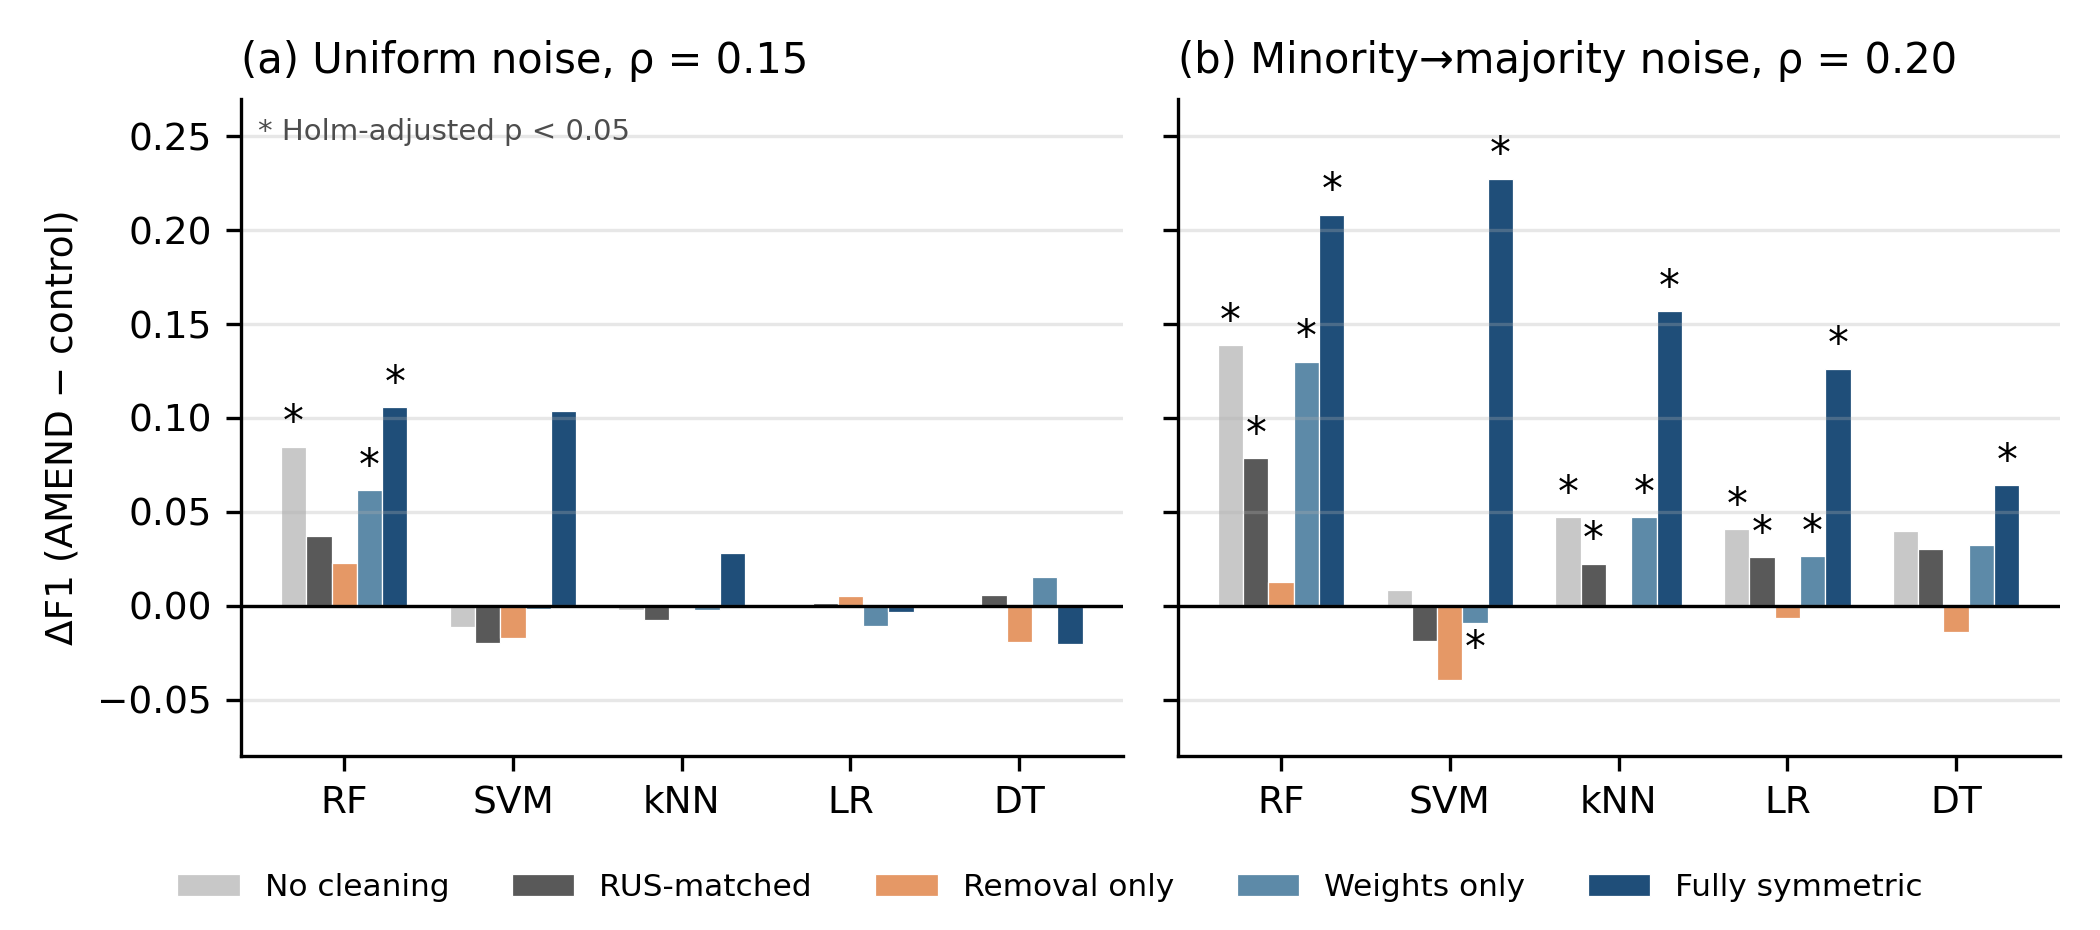
\includegraphics[width=\textwidth]{figures/fig6.png}
\caption{Controls (Experiment 7). F1 of AMEND minus each control, per classifier, mean over 13 datasets; positive values favour AMEND. For kNN, which ignores weights, removal only equals AMEND and weights only equals no cleaning. Asterisks mark Holm-adjusted $p <$ 0.05.}
\label{fig:6}
\end{figure*}

\subsection{Threshold-free ranking}\label{sec:threshold-free-ranking}

Table XI and Fig. 7a score each method's continuous suspicion score directly, with no threshold applied, so that methods are not penalised for how much they choose to remove. On this footing AMEND is the weakest of the five: mean ranking ROC-AUC 0.757 against 0.882 for IHT-score, 0.868 for CL, 0.825 for kNN-disagree and 0.795 for AUM-score, with the lowest average rank (4.31 of 5). The deficits against IHT-score ($-$0.125), CL ($-$0.111) and kNN-disagree ($-$0.068) all survive Holm correction on both ROC-AUC and average precision; the difference from AUM-score does not. Per dataset, AMEND reached 0.928 on lung and 0.904 on Carcinom but was at or below chance on CNS (0.511) and Prostate (0.449), where CL (0.532 and 0.492) and kNN-disagree (0.421 and 0.426) also failed and only AUM-score retained signal (0.617 and 0.868).

One comparison in this table bears directly on AMEND's design. kNN-disagree is the DIS component of AMEND's score used on its own, with a fixed $k$ = 5 and unprojected features. It ranked flipped samples better than the full score on 11 of the 13 datasets. Since DIS enters NS with weight 0.3 and the remaining 0.7 is the subspace term, this suggests that the geometric component dilutes the ranking, but the comparison is not matched: kNN-disagree differs from DIS in both its feature space and its $k$. Section V-I removes both differences.

\begin{table*}[!t]
\centering
\footnotesize
\caption{Threshold-free noise ranking at 15\% uniform noise (mean over 13 datasets)}
\label{tab:11}
\setlength{\tabcolsep}{3.5pt}
\begin{adjustbox}{max width=\linewidth}
\begin{tabular}{lccccccc}
\hline
Score & ROC-AUC & Rank & AP & Rank & LiftAP & $\Delta $ROC-AUC ($p_{\mathrm{Holm}}$) & $\Delta $AP ($p_{\mathrm{Holm}}$) \\
\hline
IHT-score & 0.882 & 1.54 & 0.729 & 1.38 & 5.14 & $-$0.125 ($<$0.001) & $-$0.214 ($<$0.001) \\
CL & 0.868 & 2.15 & 0.694 & 2.31 & 4.94 & $-$0.111 ($<$0.001) & $-$0.179 (0.005) \\
kNN-disagree & 0.825 & 3.15 & 0.587 & 3.31 & 4.12 & $-$0.068 (0.016) & $-$0.072 (0.009) \\
AUM-score & 0.795 & 3.85 & 0.458 & 4.15 & 3.14 & $-$0.039 (0.787) & +0.057 (0.146) \\
AMEND & 0.757 & 4.31 & 0.515 & 3.85 & 3.58 & -- & -- \\
\hline
\end{tabular}
\end{adjustbox}
\par\vspace{3pt}
\begin{minipage}{\linewidth}\scriptsize Iman--Davenport: ROC-AUC $F_{\mathrm{F}}$ = 13.54, $p <$ 0.001, critical difference 1.69; AP $F_{\mathrm{F}}$ = 13.16, $p <$ 0.001. The last two columns give AMEND minus the method, with Holm-adjusted Wilcoxon $p$.\end{minipage}
\end{table*}

\subsection{Minority-class size}\label{sec:minority-class-size}

Experiment 6 subsamples the minority class before cross-validation, so it isolates the effect of rare-class size on detection quality. Both methods degrade as the minority shrinks in absolute terms, and CL leads AMEND at every size tested (Table XII, Fig. 7b). The interesting quantity is the size of the gap: it narrows monotonically from $-$0.101 ROC-AUC at 20 minority samples to $-$0.029 at five, and reaches nominal significance only at 16 and 20 samples (uncorrected Wilcoxon $p$ = 0.014 and 0.020), not at 12 or below; by the convention of Section IV-F these remain observations. On the nine datasets present at every size from 5 to 20, AMEND's mean ROC-AUC rose from 0.740 to 0.846 as the minority was cut from 20 to five samples, improving on eight of the nine (exploratory $p$ = 0.008); CL rose from 0.841 to 0.857 on seven of nine ($p$ = 0.055). Shrinking the minority also raises the imbalance ratio and, under uniform noise, increases the share of flipped majority samples inside the minority-labelled set --- such samples often have no same-label neighbour and receive the maximum score NS = 1 --- so this trend cannot be credited to the geometry alone. The defensible statement is that AMEND's disadvantage relative to CL disappears in the smallest-minority regime, not that it reverses.

\begin{table*}[!t]
\centering
\footnotesize
\caption{Ranking ROC-AUC as the minority class is subsampled (Experiment 6)}
\label{tab:12}
\setlength{\tabcolsep}{3.5pt}
\begin{adjustbox}{max width=\linewidth}
\begin{tabular}{lcccccc}
\hline
Minority size & $N$ & AMEND ROC-AUC & CL ROC-AUC & $\Delta $ (AMEND $-$ CL) & W/L & $p$ \\
\hline
5 & 13 & 0.854 & 0.883 & $-$0.029 & 2/11 & 0.168 \\
8 & 12 & 0.827 & 0.872 & $-$0.045 & 2/10 & 0.233 \\
12 & 10 & 0.779 & 0.853 & $-$0.073 & 2/8 & 0.084 \\
16 & 10 & 0.755 & 0.849 & $-$0.093 & 2/8 & 0.014 \\
20 & 9 & 0.740 & 0.841 & $-$0.101 & 1/8 & 0.020 \\
30 & 3 & 0.715 & 0.804 & $-$0.089 & 0/3 & n/a \\
45 & 2 & 0.619 & 0.713 & $-$0.094 & 0/2 & n/a \\
\hline
\end{tabular}
\end{adjustbox}
\par\vspace{3pt}
\begin{minipage}{\linewidth}\scriptsize $N$: datasets with at least that many minority samples. W/L: datasets on which AMEND scored higher/lower than CL. $p$: two-sided Wilcoxon, not corrected across sizes; sizes with fewer than five non-zero differences are not tested.\end{minipage}
\end{table*}

\begin{figure*}[!t]
\centering
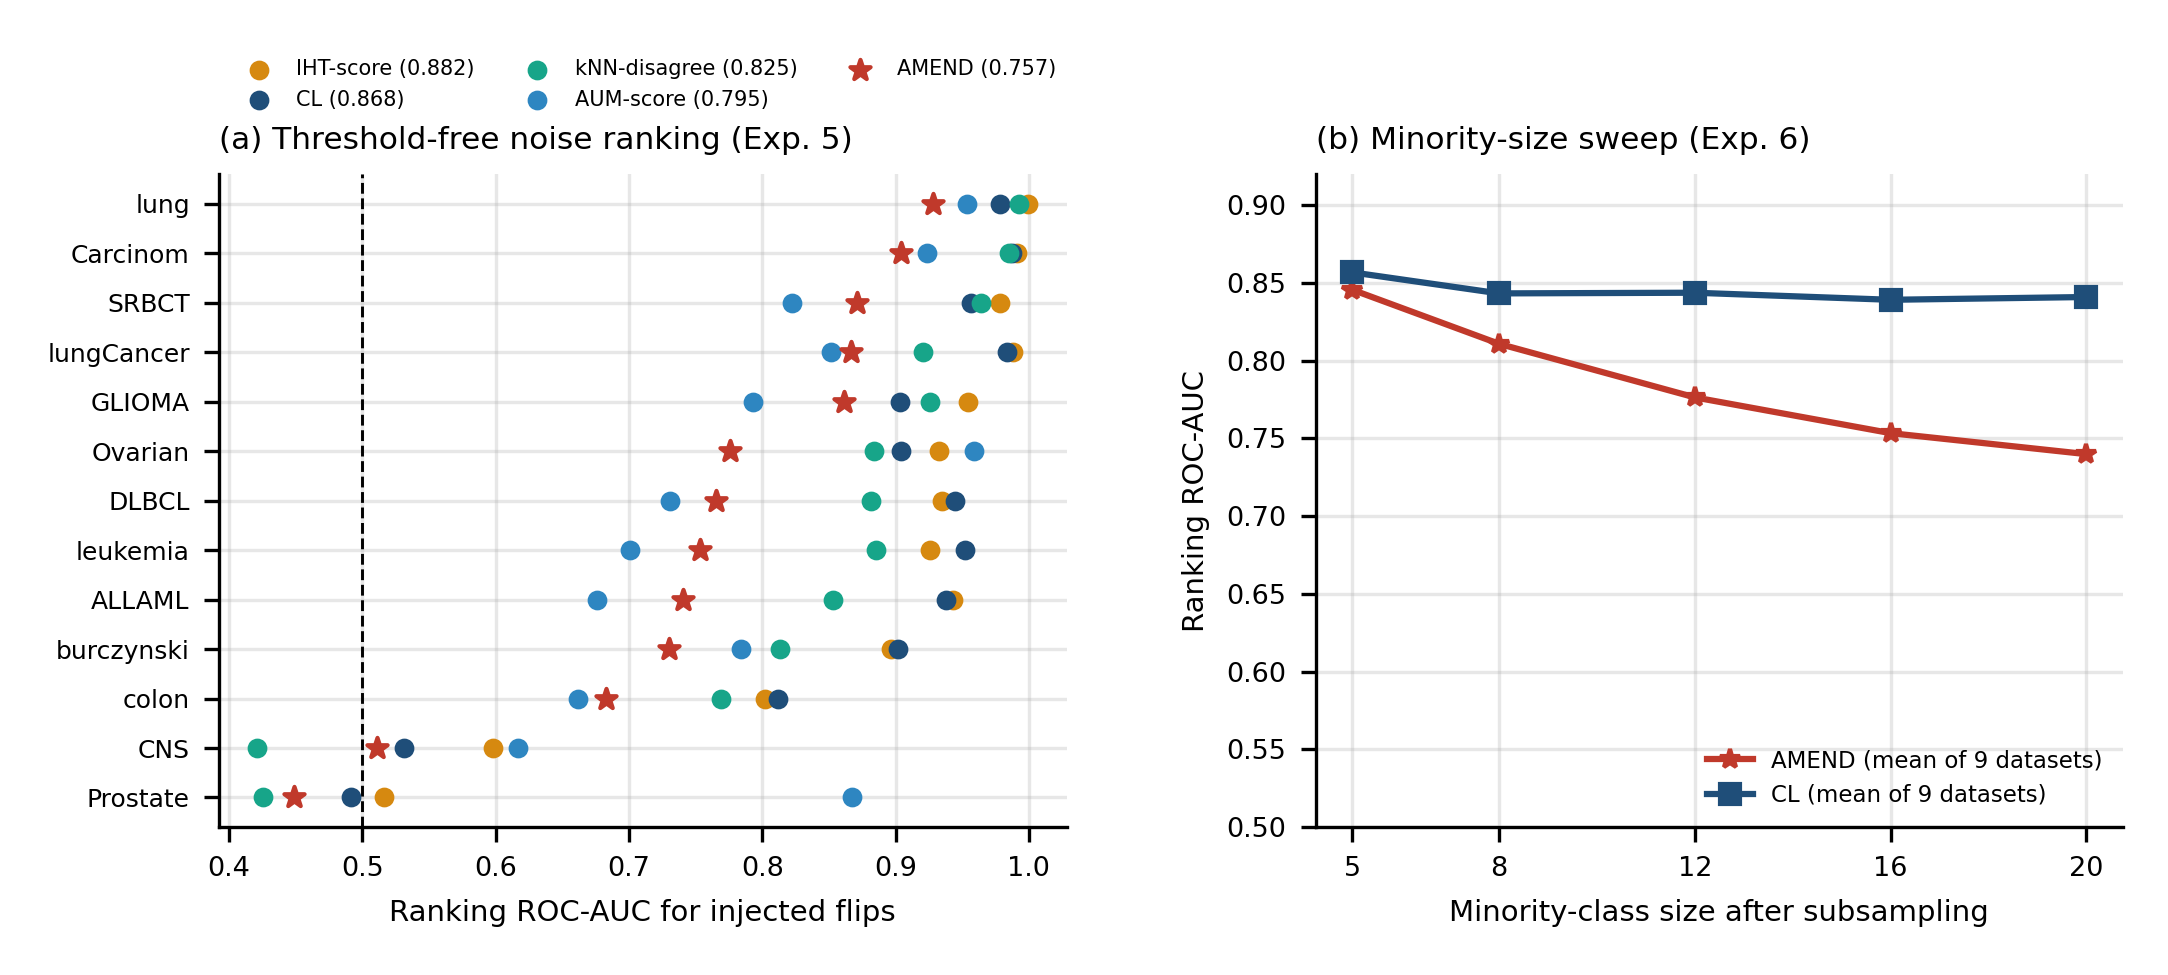
\includegraphics[width=\textwidth]{figures/fig7.png}
\caption{(a) Ranking ROC-AUC of five noise scores per dataset at 15\% uniform noise; the dashed line marks chance and legend values are means over datasets. (b) Ranking ROC-AUC as the minority class is subsampled, averaged over the datasets available at every size.}
\label{fig:7}
\end{figure*}

\subsection{Contribution of the subspace term: agree-weight sweep}\label{sec:contribution-of-the-subspace-term-agree-weight-sweep}

Experiment 8 answers the question that the ablation and the ranking analysis could approach only indirectly. It varies $w$ in (7) from 0, where the score is the subspace term 1 $-$ SCS alone, to 1, where it is neighbour-label disagreement alone, with the projection, the standardisation, $k$ and the rest of the pipeline unchanged (Table XIII, Fig. 8). The ranking quality of NS rose steadily with $w$, from ROC-AUC 0.637 at $w$ = 0 to 0.757 at the default $w$ = 0.3 and 0.807 at $w$ = 1, and the Friedman test rejected equality across the seven settings ($F_{\mathrm{F}}$ = 29.68, $p <$ 0.001). The default ranked significantly worse than $w$ = 0.5, 0.7 and 1, by 0.041 to 0.051 (lower on 12 or 13 of 13 datasets; Holm $p \le $ 0.003), and significantly better than $w$ = 0, 0.1 and 0.2. Twelve of the 13 datasets followed the same rising curve; on the remaining one, Prostate, every setting ranked below chance. Average precision told the same story, except that $w$ = 1 and the default did not differ (Holm $p$ = 1.000). The best setting on both ranking measures was $w$ = 0.7, which did not differ from $w$ = 1 on ROC-AUC (+0.001; post-hoc $p$ = 0.42).

\begin{table*}[!t]
\centering
\footnotesize
\caption{Agree-weight sweep at 15\% uniform noise (Experiment 8)}
\label{tab:13}
\setlength{\tabcolsep}{3.5pt}
\begin{adjustbox}{max width=\linewidth}
\begin{tabular}{lcccccccccc}
\hline
$w$ & Ranking ROC-AUC (rank) & $\Delta $ ROC-AUC ($p_{\mathrm{Holm}}$) & Ranking AP (rank) & F1 (rank) & $\Delta $F1 ($p_{\mathrm{Holm}}$) & G-mean & $\tau $ & Removal & Prec. & FRR \\
\hline
0 & 0.637 (6.54) & \textbf{$-$0.120 (0.003)} & 0.408 (6.46) & 0.580 (5.38) & $-$0.044 (0.239) & 0.655 & 0.458 & 0.157 & 0.098 & 0.169 \\
0.1 & 0.680 (5.69) & \textbf{$-$0.077 (0.003)} & 0.447 (5.62) & 0.594 (4.69) & $-$0.030 (0.439) & 0.678 & 0.389 & 0.135 & 0.119 & 0.144 \\
0.2 & 0.722 (4.85) & \textbf{$-$0.035 (0.003)} & 0.485 (4.54) & 0.612 (4.46) & $-$0.012 (0.439) & 0.698 & 0.286 & 0.100 & 0.156 & 0.103 \\
0.3 (default) & 0.757 (4.08) & -- & 0.515 (3.31) & 0.624 (3.85) & -- & 0.707 & 0.237 & 0.083 & 0.179 & 0.083 \\
0.5 & 0.798 (3.08) & \textbf{+0.041 (0.002)} & 0.555 (2.38) & 0.628 (3.00) & +0.004 (0.439) & 0.714 & 0.273 & 0.094 & 0.172 & 0.092 \\
0.7 & 0.808 (1.65) & \textbf{+0.051 (0.003)} & 0.567 (1.62) & 0.628 (2.46) & +0.004 (0.402) & 0.719 & 0.332 & 0.114 & 0.163 & 0.113 \\
1 & 0.807 (2.12) & \textbf{+0.050 (0.001)} & 0.526 (4.08) & 0.619 (4.15) & $-$0.005 (0.439) & 0.707 & 0.340 & 0.065 & 0.209 & 0.061 \\
\hline
\end{tabular}
\end{adjustbox}
\par\vspace{3pt}
\begin{minipage}{\linewidth}\scriptsize Means over 13 datasets (and five classifiers for F1 and G-mean). Ranking ROC-AUC and AP score NS against the injected flips; average Friedman ranks over the seven settings are in parentheses (lower is better; critical difference 2.50). $\Delta $: setting minus the default $w$ = 0.3, with Holm-adjusted Wilcoxon $p$; bold marks $p <$ 0.05. Iman--Davenport: ROC-AUC $F_{\mathrm{F}}$ = 29.68, AP $F_{\mathrm{F}}$ = 20.75, F1 $F_{\mathrm{F}}$ = 3.29 ($p$ = 0.006). Removal: removal rate; Prec.: noise precision of removals.\end{minipage}
\end{table*}

The subspace term is not devoid of signal. On its own it ranked flipped samples above chance on 12 of the 13 datasets (mean 0.637; post-hoc Wilcoxon against 0.5, $p <$ 0.001). It was, however, weaker than disagreement alone on 12 of 13 datasets, and mixing it in at weight 0.7, as the default does, lowered the ranking below that of disagreement alone on all 13 (Holm $p$ = 0.001).

The end task was much less sensitive to $w$. Mean F1 ranged from 0.580 at $w$ = 0 to 0.628 at $w$ = 0.7, and although the Friedman test detected a difference across settings ($F_{\mathrm{F}}$ = 3.29, $p$ = 0.006), no setting differed from the default after Holm correction (smallest adjusted $p$ = 0.239, for $w$ = 0). The subspace-only score was the weakest cleaner end to end: it set the largest threshold ($\tau $ = 0.458) and removed 15.7\% of the training fold with the lowest removal precision (0.098) and the highest false-removal rate (0.169). Disagreement alone was the most conservative setting (removal rate 0.065, FRR 0.061, removal precision 0.209) and gave F1 0.619. In a single uncorrected post-hoc comparison, $w$ = 0.7 had higher F1 than $w$ = 1 on 10 of 13 datasets (+0.009, $p$ = 0.021), so a small subspace admixture may help the end task slightly even though it does not help the ranking; we treat this as an observation.

With projection and $k$ matched, then, neighbour-label disagreement ranks wrong labels better than local subspace coherence, and the default mixture ranks them worse than disagreement alone. The subspace term carries some signal, but on these datasets the disagreement term it is mixed with dominates it.

\begin{figure*}[!t]
\centering
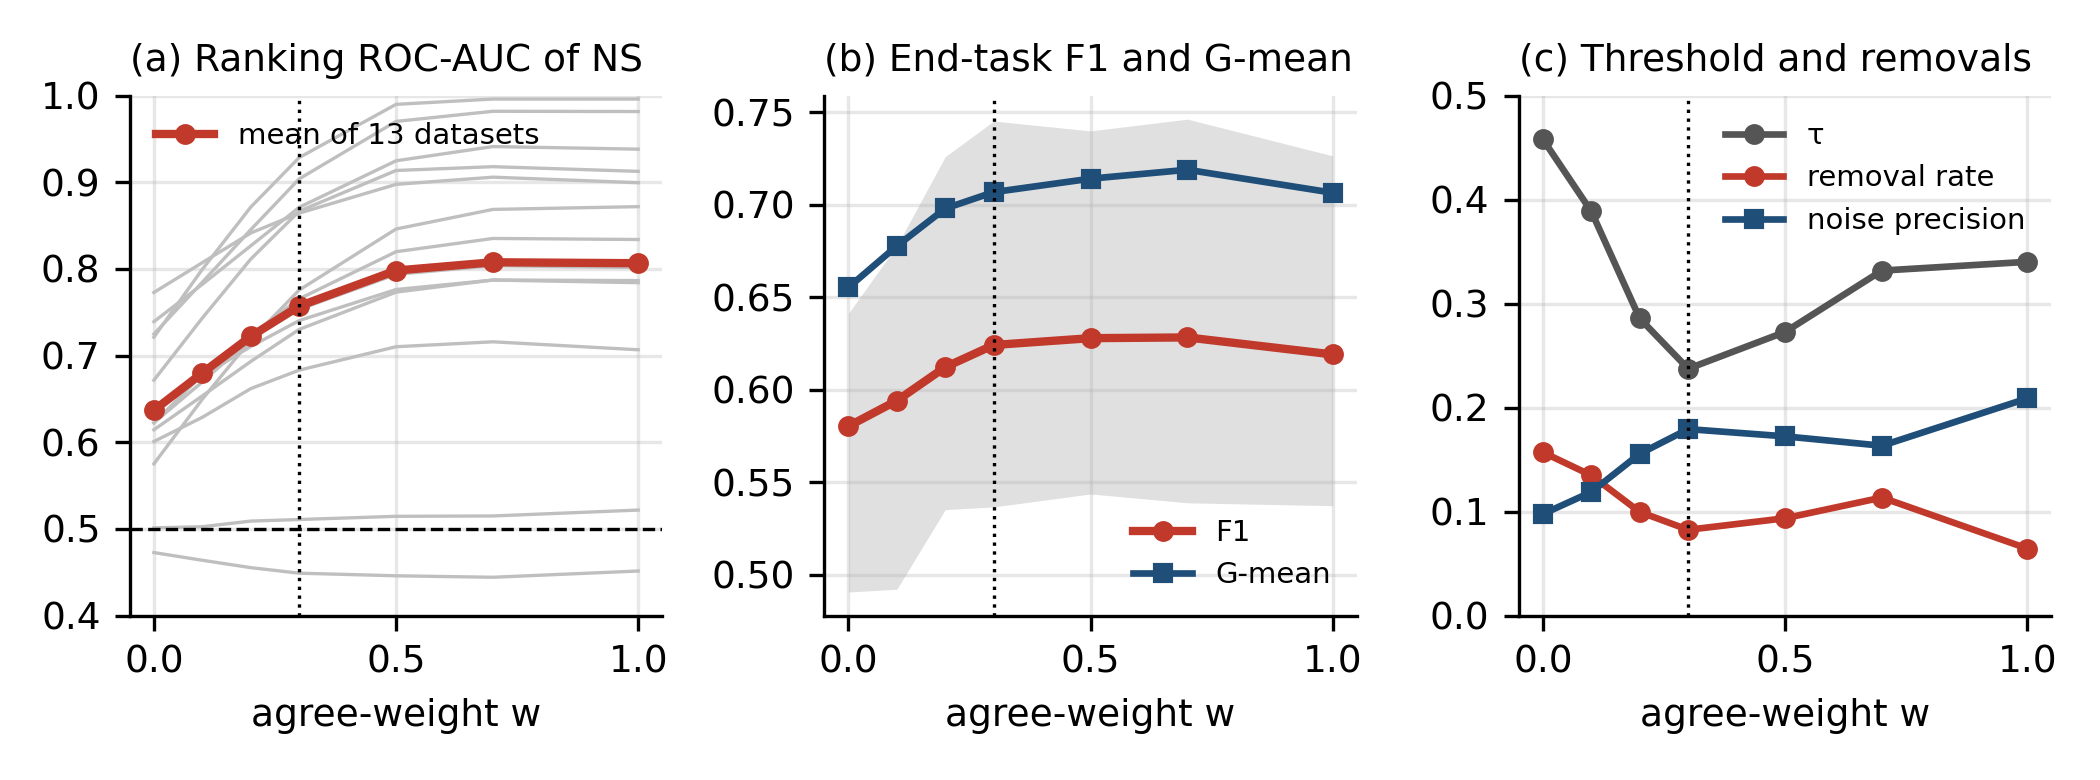
\includegraphics[width=\textwidth]{figures/fig8.png}
\caption{Agree-weight sweep at 15\% uniform noise (Experiment 8). $w$ = 0 uses the subspace term alone, $w$ = 1 neighbour-label disagreement alone, and the dotted line marks the default $w$ = 0.3. (a) Ranking ROC-AUC of NS against the injected flips, per dataset (grey) and mean (red); the dashed line marks chance. (b) End-task F1 and G-mean, means over datasets and classifiers; the band is the interquartile range of F1 over datasets. (c) Estimated contamination $\tau $, removal rate and noise precision of removals.}
\label{fig:8}
\end{figure*}

\subsection{Ablation}\label{sec:ablation}

Table XIV varies one factor at a time around AMEND's default configuration; the label-disagreement weight $w$, the Gaussian-mixture threshold and anchored rescue were held fixed in every row ($w$ is varied separately in Section V-I). No statistical tests were run on the ablation, so all statements here are observations. Mean F1 across configurations ranged from 0.600 to 0.628 against 0.611 for no cleaning, and ROC-AUC from 0.817 to 0.823 against 0.826, so the control had higher ROC-AUC than every configuration tried.

The choice between the two geometric terms mattered little for the end task: the full $\alpha $ sweep from 0 (FNS only) to 1 (SCS only, which is the default score) spans just 0.004 F1, from 0.620 to 0.624. The $\alpha $ = 1 row is numerically identical to the default row because setting $\alpha $ = 1 is what disables the FNS term. One quantity does vary monotonically with $\alpha $: the false-removal rate falls from 0.113 at $\alpha $ = 0 to 0.083 at $\alpha $ = 1, and removal precision rises from 0.155 to 0.179, so the subspace-coherence term makes the cleaner more cautious and its removals cleaner without changing end-task F1 appreciably. The rows for $r$ = 5 and $r$ = 8 are nearly identical because $r$ is capped at $k -$ 1 (Section V-K). Larger neighbourhoods lowered F1 (0.612 at $k$ = 12, 0.602 at $k$ = 20), but the skip rule left 7.7\% and 33.5\% of folds uncleaned at those settings, so those rows mix cleaning with no cleaning. Class-symmetric thresholds cut FRR to 0.038 but also cut F1 to 0.600 and G-mean to 0.673, the largest end-task effect in the table. That row pools the thresholds but still never deletes a minority-labelled sample, so it isolates the asymmetry of the thresholds; the asymmetry of removal is tested by the fully symmetric variant of Section V-F, where its effect was larger still. A fixed configuration with $k$ = 5, $r$ = 5 and the older projection heuristic gave F1 0.626 and ROC-AUC 0.823, so the automatic parameter selection bought convenience rather than accuracy.

\begin{table*}[!t]
\centering
\footnotesize
\caption{Ablation at 15\% uniform noise (means over 13 datasets and five classifiers)}
\label{tab:14}
\setlength{\tabcolsep}{3.5pt}
\begin{tabular}{>{\raggedright\arraybackslash}p{0.4197\dimexpr\linewidth-16\tabcolsep\relax}>{\raggedright\arraybackslash}p{0.0631\dimexpr\linewidth-16\tabcolsep\relax}>{\raggedright\arraybackslash}p{0.0725\dimexpr\linewidth-16\tabcolsep\relax}>{\raggedright\arraybackslash}p{0.0631\dimexpr\linewidth-16\tabcolsep\relax}>{\raggedright\arraybackslash}p{0.1141\dimexpr\linewidth-16\tabcolsep\relax}>{\raggedright\arraybackslash}p{0.1064\dimexpr\linewidth-16\tabcolsep\relax}>{\raggedright\arraybackslash}p{0.0631\dimexpr\linewidth-16\tabcolsep\relax}>{\raggedright\arraybackslash}p{0.0979\dimexpr\linewidth-16\tabcolsep\relax}}
\hline
Configuration & F1 & G-mean & AUC & Noise prec. & Noise rec. & FRR & Skip rate \\
\hline
No cleaning (control) & 0.611 & 0.690 & 0.826 & -- & -- & -- & -- \\
AMEND default (k, r, p automatic; SCS only; asymmetric) & 0.624 & 0.707 & 0.819 & 0.179 & 0.087 & 0.083 & 0.000 \\
k = 5 & 0.624 & 0.704 & 0.821 & 0.178 & 0.084 & 0.078 & 0.002 \\
k = 8 & 0.618 & 0.699 & 0.819 & 0.182 & 0.091 & 0.088 & 0.014 \\
k = 12 & 0.612 & 0.695 & 0.818 & 0.169 & 0.099 & 0.099 & 0.077 \\
k = 20 & 0.602 & 0.686 & 0.818 & 0.118 & 0.075 & 0.076 & 0.335 \\
r = 2 & 0.628 & 0.708 & 0.818 & 0.171 & 0.103 & 0.100 & 0.000 \\
r = 3 & 0.626 & 0.706 & 0.819 & 0.178 & 0.092 & 0.089 & 0.000 \\
r = 5 & 0.624 & 0.707 & 0.819 & 0.179 & 0.087 & 0.083 & 0.000 \\
r = 8 & 0.624 & 0.707 & 0.819 & 0.179 & 0.086 & 0.082 & 0.000 \\
$\alpha $ = 0 (FNS only) & 0.620 & 0.703 & 0.818 & 0.155 & 0.110 & 0.113 & 0.000 \\
$\alpha $ = 0.25 & 0.621 & 0.708 & 0.818 & 0.162 & 0.106 & 0.105 & 0.000 \\
$\alpha $ = 0.5 (SCS + FNS) & 0.624 & 0.709 & 0.820 & 0.170 & 0.098 & 0.091 & 0.000 \\
$\alpha $ = 0.75 & 0.623 & 0.710 & 0.820 & 0.174 & 0.089 & 0.083 & 0.000 \\
$\alpha $ = 1 (SCS only; the default score) & 0.624 & 0.707 & 0.819 & 0.179 & 0.087 & 0.083 & 0.000 \\
Class-symmetric thresholds & 0.600 & 0.673 & 0.821 & 0.147 & 0.045 & 0.038 & 0.000 \\
Fixed k = 5, r = 5, legacy projection & 0.626 & 0.704 & 0.823 & 0.175 & 0.076 & 0.067 & 0.002 \\
\hline
\end{tabular}
\par\vspace{3pt}
\begin{minipage}{\linewidth}\scriptsize Each row changes one factor relative to the default configuration; $w$ = 0.3, Gaussian-mixture thresholding and anchored rescue are fixed throughout. The class-symmetric row pools the thresholds of (9) but keeps removal restricted to majority-labelled samples.\end{minipage}
\end{table*}

\subsection{Internal state of AMEND}\label{sec:internal-state-of-amend}

Experiment 11 records what AMEND does inside each fold (Table XV). Three observations bear on the interpretation of the results above. First, the local subspace usually spans the whole neighbourhood. At 15\% uniform noise the realised neighbourhood size averaged 5.2 and the local rank 4.1, and $r$ sat at its cap $k -$ 1 in 88.5\% of folds; on ten datasets it did so in every fold, and it stayed below the cap in every fold only on Ovarian, where $k \approx $ 9. The covariance of $k$ centred neighbours has rank at most $k -$ 1, so with $r$ = $k -$ 1 the estimated subspace is the span of the centred neighbourhood itself. SCS then compares the spans of two neighbourhoods, which agree largely when the neighbourhoods share points, rather than testing whether the samples lie on a common low-dimensional structure. This is consistent with the weak ranking of the subspace term in Section V-I.

Second, the threshold does not track the noise. The estimated contamination $\tau $ averaged 0.304 on clean data and 0.237 at 15\% uniform noise, and AMEND removed 12.0\% and 8.3\% of the training fold in the two conditions, so both quantities were larger with no injected noise than with it. On clean data only 49.7\% of retained samples kept weight 1, and 31.5\% received $\omega  \le $ 0.5.

Third, the rebalancing depends on the condition. On clean data AMEND lowered the effective imbalance ratio on 11 of 13 datasets, from 4.52 to 2.82 on average (median ratio of after to before 0.76), and sharply on the most imbalanced ones (Carcinom 14.76 to 5.62, lung 9.15 to 2.55). Under 20\% majority$\rightarrow $minority noise it lowered the ratio on 12 of 13 datasets (1.75 to 1.46). At 15\% uniform noise the mean ratio was unchanged (2.34 before and after): majority removals were offset by the quarantine of minority-labelled samples, many of them flipped majority samples, and on five datasets, including Carcinom (4.11 to 4.92) and GLIOMA (3.25 to 4.38), the effective imbalance increased. Under 20\% minority$\rightarrow $majority noise the mean ratio fell from 6.38 to 5.68, on 7 of 13 datasets. AMEND therefore rebalances most strongly on clean and majority$\rightarrow $minority-corrupted data, where the noise sweep found no end-task benefit (Table VI), and only moderately in the regime where it helps most.

\begin{table*}[!t]
\centering
\footnotesize
\caption{Internal state of AMEND (Experiment 11; no classifiers trained)}
\label{tab:15}
\setlength{\tabcolsep}{3.5pt}
\begin{adjustbox}{max width=\linewidth}
\begin{tabular}{lcccccccccc}
\hline
Dataset & $k$ & $r$ & At cap & $p$ & $\tau $ & Removal & $\omega $ = 1 & $\omega  \le $ 0.5 & Eff. IR before & Eff. IR after \\
\hline
ALLAML & 4.86 & 3.86 & 100\% & 56.6 & 0.258 & 0.082 & 0.617 & 0.182 & 1.55 & 1.33 \\
burczynski & 5.52 & 4.52 & 100\% & 100.6 & 0.346 & 0.123 & 0.453 & 0.319 & 2.35 & 1.62 \\
Carcinom & 5.22 & 4.22 & 100\% & 128.0 & 0.174 & 0.073 & 0.670 & 0.199 & 4.11 & 4.92 \\
CNS & 4.16 & 3.16 & 100\% & 47.0 & 0.280 & 0.093 & 0.571 & 0.225 & 1.74 & 1.48 \\
colon & 4.26 & 3.26 & 100\% & 48.6 & 0.309 & 0.098 & 0.542 & 0.223 & 1.57 & 1.21 \\
DLBCL & 4.46 & 3.46 & 100\% & 60.6 & 0.196 & 0.072 & 0.700 & 0.155 & 2.10 & 1.88 \\
GLIOMA & 3.12 & 2.12 & 100\% & 39.0 & 0.218 & 0.089 & 0.617 & 0.218 & 3.25 & 4.38 \\
leukemia & 4.86 & 3.86 & 100\% & 56.6 & 0.283 & 0.091 & 0.581 & 0.216 & 1.55 & 1.21 \\
lung & 6.00 & 4.90 & 90\% & 128.0 & 0.138 & 0.056 & 0.740 & 0.150 & 3.48 & 3.88 \\
lungCancer & 6.28 & 4.88 & 60\% & 128.0 & 0.164 & 0.062 & 0.711 & 0.143 & 2.74 & 2.95 \\
Ovarian & 9.02 & 7.02 & 0\% & 128.0 & 0.164 & 0.051 & 0.773 & 0.102 & 1.51 & 1.36 \\
Prostate & 5.98 & 4.98 & 100\% & 80.6 & 0.337 & 0.093 & 0.523 & 0.251 & 1.16 & 0.77 \\
SRBCT & 3.94 & 2.94 & 100\% & 65.4 & 0.220 & 0.089 & 0.617 & 0.214 & 3.35 & 3.37 \\
\textbf{Mean, uniform 0.15} & \textbf{5.21} & \textbf{4.09} & \textbf{88.5\%} & \textbf{82.1} & \textbf{0.237} & \textbf{0.083} & \textbf{0.624} & \textbf{0.200} & \textbf{2.34} & \textbf{2.34} \\
Mean, clean data & 4.43 & 3.35 & 92.3\% & 82.1 & 0.304 & 0.120 & 0.497 & 0.315 & 4.52 & 2.82 \\
Mean, min$\rightarrow $maj 0.20 & 4.03 & 2.96 & 92.6\% & 82.1 & 0.265 & 0.112 & 0.541 & 0.283 & 6.38 & 5.68 \\
Mean, maj$\rightarrow $min 0.20 & 5.70 & 4.49 & 78.6\% & 82.1 & 0.263 & 0.084 & 0.605 & 0.214 & 1.75 & 1.46 \\
\hline
\end{tabular}
\end{adjustbox}
\par\vspace{3pt}
\begin{minipage}{\linewidth}\scriptsize Per-dataset rows: 15\% uniform noise, means over 50 folds. $k$, $r$: realised neighbourhood size and local rank; at cap: share of folds with $r$ = $k -$ 1; $p$: working projection width; $\omega $ = 1 and $\omega  \le $ 0.5: shares of retained samples; Eff. IR: sum of weights over majority-labelled samples divided by the sum over minority-labelled samples, on the observed labels, before and after cleaning.\end{minipage}
\end{table*}

\subsection{Runtime}\label{sec:runtime}

On the 13 real datasets, where $d$ ranges from 2000 to 22 283, AMEND was the second-fastest method: 0.225 s per training fold against 0.015 s for ENN, 0.032 s for AllKNN, 1.62 s for CL, 2.22 s for IHT and 45.95 s for AUM (Table V). AMEND was thus about seven times faster than CL on the data it is intended for, because it needs no cross-validated model fitting. On synthetic data (Table XVI) its time grew linearly with $n$, from 0.16 s at $n$ = 200 to 3.20 s at $n$ = 4000 with $d$ = 50 (log--log slope 1.00). Against $d$ at $n$ = 1000 it took 0.28 s at $d$ = 20 and about 1.5 s from $d$ = 300 onwards, the plateau expected from the projection cap at $p$ = 128; CL was faster in absolute terms on this narrow synthetic data (0.05 to 0.34 s), which is the opposite of the ordering on the real high-dimensional datasets. The setting $n$ = 1000, $d$ = 50 appears in both sweeps and was timed at 0.74 s and 1.05 s, so single measurements vary by tens of percent.

\begin{table}[!t]
\centering
\footnotesize
\caption{AMEND cleaning time on synthetic data (median of three runs, one seed)}
\label{tab:16}
\setlength{\tabcolsep}{3.5pt}
\begin{adjustbox}{max width=\linewidth}
\begin{tabular}{lccc}
\hline
$n$ ($d$ = 50) & Time (s) & $d$ ($n$ = 1000) & Time (s) \\
\hline
200 & 0.16 & 20 & 0.28 \\
500 & 0.35 & 50 & 1.05 \\
1000 & 0.74 & 100 & 1.04 \\
2000 & 1.51 & 300 & 1.53 \\
4000 & 3.20 & 1000 & 1.54 \\
\hline
\end{tabular}
\end{adjustbox}
\end{table}

\subsection{Behaviour in the high-dimensional regime}\label{sec:behaviour-in-the-high-dimensional-regime}

Every dataset in this study has at least 2000 features and a feature-to-sample ratio between 16 and 175, so all results above were obtained in the high-dimensional small-sample regime, and none of them speaks to low-dimensional data. Two further analyses look at the regime directly.

First, the composition of AMEND's input is entirely determined by the projection in this regime. Because every dataset has $d \ge $ 2000 and the Johnson--Lindenstrauss bound exceeds 128 at these sample sizes, the projection was applied in every fold and the working width was min(128, $n -$ 1): 128 for Carcinom, lung, lungCancer and Ovarian and between 39 and 101 for the other nine datasets. AMEND therefore never operates on more than 128 dimensions regardless of whether the input has 2000 or 22 283 features, which is what bounds both its cost and its variance in $d$. The runtime measurements bear this out, with cleaning time flat from $d$ = 300 to $d$ = 1000 (Fig. 9b) and 0.225 s per fold on real data with up to 22 283 features.

Second, as an exploratory observation, AMEND's standing relative to CL varies systematically with the feature-to-sample ratio. Across the 13 datasets the per-dataset F1 difference between AMEND and CL at 15\% uniform noise correlates with $d$/$n$ (Spearman $\rho $ = 0.588, $p$ = 0.035; Fig. 9a). AMEND led CL on five datasets: the two with the largest ratios (burczynski and CNS), GLIOMA, colon and the most balanced one, Prostate; its largest deficits were on lung and Carcinom, which have among the lowest ratios. The same correlation against $d$ alone is not significant ($\rho $ = 0.041, $p$ = 0.894), and the correlation of AMEND's advantage over no cleaning with either quantity is not significant ($\rho $ = 0.165 and 0.104). This is a single uncorrected test on 13 points and should be treated as a hypothesis for a larger study, not as a demonstration; what it does not support is any claim that AMEND is generally preferable on wide data.

\begin{figure*}[!t]
\centering
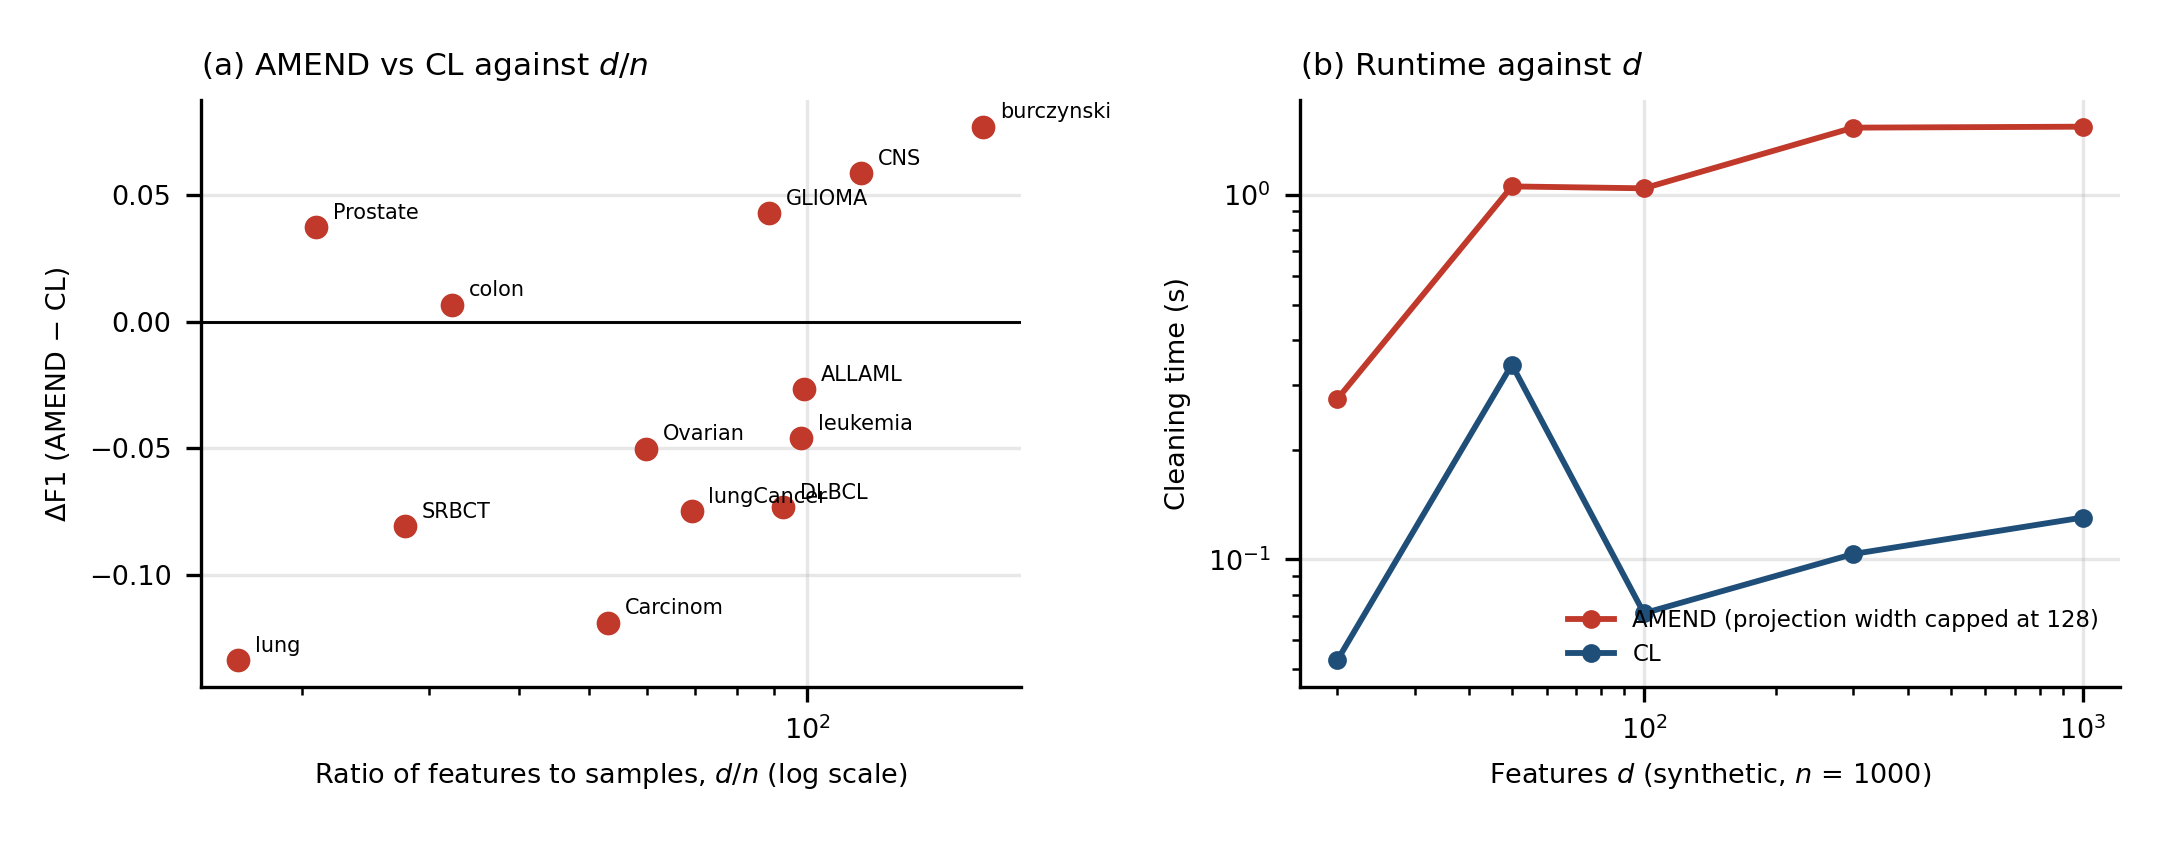
\includegraphics[width=\textwidth]{figures/fig9.png}
\caption{The high-dimensional regime. (a) Per-dataset F1 difference between AMEND and CL at 15\% uniform noise against the feature-to-sample ratio $d$/$n$ (Spearman $\rho $ = 0.588, $p$ = 0.035, exploratory). (b) Cleaning time against the number of features on synthetic data with $n$ = 1000; AMEND's curve flattens once $d$ exceeds the projection cap.}
\label{fig:9}
\end{figure*}

\subsection{Summary of evidence}\label{sec:summary-of-evidence}

Table XVII grades every claim the experiments bear on. The statistically supported positive claims concern the asymmetric rule in the regime it targets: gains over no cleaning under minority$\rightarrow $majority and minority instance-dependent noise, removals that beat matched random undersampling there, and a clear loss when the asymmetry is removed; random forests benefit most. The negative findings are as firm: CL is the better detector and ranker in every condition, the end-task effect under uniform noise cannot be separated from rebalancing, the soft weights add nothing measurable to the removals, and two mechanisms of the original design, a noise-adaptive threshold and a subspace term that adds signal, are not supported.

\begin{table*}[!t]
\centering
\footnotesize
\caption{Evidence summary}
\label{tab:17}
\setlength{\tabcolsep}{3.5pt}
\begin{tabular}{>{\raggedright\arraybackslash}p{0.3939\dimexpr\linewidth-6\tabcolsep\relax}>{\raggedright\arraybackslash}p{0.4535\dimexpr\linewidth-6\tabcolsep\relax}>{\raggedright\arraybackslash}p{0.1526\dimexpr\linewidth-6\tabcolsep\relax}}
\hline
Claim & Evidence & Status \\
\hline
Removal asymmetry improves the end task & Fully symmetric variant worse for all five classifiers under minority$\rightarrow $majority noise, $p_{\mathrm{Holm}} \le $ 0.028, and for RF under uniform noise (Table X) & Supported (for) \\
F1 gain over no cleaning under minority$\rightarrow $majority noise, $\rho $ = 0.05--0.40 & $\Delta $F1 +0.023 to +0.059; 12--13 of 13 datasets; $p_{\mathrm{Holm}} \le $ 0.027 (Table VI) & Supported (for) \\
G-mean gain over no cleaning under minority$\rightarrow $majority noise, $\rho $ = 0.10--0.40 & +0.035 to +0.059; $p_{\mathrm{Holm}} \le $ 0.029 (Table VI) & Supported (for) \\
Removals chosen better than matched random undersampling under minority$\rightarrow $majority noise & F1 +0.079 (RF), +0.026 (LR), +0.022 (kNN), $p_{\mathrm{Holm}} \le $ 0.007; DT and SVM not significant (Table X) & Supported (for, 3 of 5 classifiers) \\
F1 gain over no cleaning under instance-dependent noise & +0.011 to +0.046 in all eight conditions; $p_{\mathrm{Holm}} \le $ 0.015 in four (Table VII) & Supported (for, 4 of 8 conditions) \\
F1 above CL under minority instance-dependent noise & +0.036 at $\rho $ = 0.30, 11/13 datasets, $p_{\mathrm{Holm}}$ = 0.020; G-mean also at $\rho $ = 0.20 (Table VII) & Supported (for, post-hoc) \\
Best F1 and G-mean of seven methods with random forests & F1 0.666, rank 2.23/7, $p$ = 0.007; G-mean beats CL by +0.068, $p_{\mathrm{Holm}}$ = 0.010 (Tables III, IV) & Supported (for) \\
Lowest false-removal rate of every method that removes a comparable share of data & FRR 0.083 vs 0.172 (CL) to 0.411 (ENN); $p_{\mathrm{Holm}} \le $ 0.002 (Table V) & Supported (for) \\
More precise removals than ENN, AllKNN, IHT and random majority removal & +0.054 to +0.081 vs editors, $p_{\mathrm{Holm}} \le $ 0.012; 0.179 vs 0.060 for RUS-matched, 11/13 datasets (Tables V, IX) & Supported (for) \\
Lower FPR and higher F1 than ENN, AllKNN and IHT & FPR for all five classifiers; F1 for LR; $p_{\mathrm{Holm}} \le $ 0.040 (Table IV) & Supported (for) \\
Cost bounded in the number of features & Working width $\le $ 128 for $d$ = 2000--22 283; 0.225 s/fold vs 1.62 s for CL; flat beyond $d$ = 300 (Sections V-L, V-M) & Observation (for) \\
Matches CL under minority$\rightarrow $majority noise & $\Delta $F1 +0.012 to +0.037, 6/7 to 10/3 datasets, no $p_{\mathrm{Holm}} <$ 0.05 (Table VI); within +0.026 of CL-matched, none significant (Table VIII) & Observation (neutral) \\
Gap to CL narrows as the minority class shrinks & $\Delta  -$0.101 at 20 samples to $-$0.029 at five; significant only at 16 and 20 (Table XII) & Observation (neutral) \\
A matched base model strengthens CL & CL-matched mean F1 0.633 vs 0.654 (uniform), 0.606 vs 0.601 (minority$\rightarrow $majority) (Table VIII) & Not supported \\
Advantage over CL grows with $d$/$n$ & Spearman $\rho $ = 0.588, $p$ = 0.035, single exploratory test (Section V-M) & Observation (for, weak) \\
Lower mean F1 and ROC-AUC than CL at 15\% uniform noise & 0.624 vs 0.654 and 0.819 vs 0.844; significant for DT (Tables III, IV) & Partly supported (against) \\
Far weaker noise detection than CL & Precision $-$0.341, recall $-$0.654, noise F1 $-$0.487, $p_{\mathrm{Holm}} \le $ 0.001 (Table V); lower precision and recall under instance-dependent noise (Table VII) & Supported (against) \\
Higher test-set FPR than no cleaning, CL and AUM & All five classifiers; $p_{\mathrm{Holm}} \le $ 0.008 (Table IV) & Supported (against) \\
Weakest noise ranking of the five scores compared & ROC-AUC 0.757; deficits to IHT-score, CL, kNN-disagree $p_{\mathrm{Holm}} \le $ 0.016 (Table XI) & Supported (against) \\
End-task gain beyond rebalancing under uniform noise & No F1 difference from RUS-matched for any classifier (largest +0.037, $p_{\mathrm{Holm}}$ = 0.172); G-mean +0.050 (RF) and $-$0.055 (SVM) (Table X) & Not supported \\
Soft weights add to removal & Removal only: mean F1 0.626 and 0.629 vs 0.624 and 0.619 for AMEND; no F1 difference significant (Tables IX, X) & Not supported \\
F1 loss under majority$\rightarrow $minority noise & $-$0.006 to $-$0.055 vs no cleaning, $-$0.016 to $-$0.094 vs CL; both significant at $\rho $ = 0.30 (Table VI) & Partly supported (against) \\
No ROC-AUC improvement over no cleaning & $\Delta  -$0.014 to $-$0.001 at 15\% uniform noise; below no cleaning in all eight instance-dependent conditions; none significant (Tables IV, VII, XIV) & Observation (against) \\
Removal rate follows the noise level & 7.6--12.0\% removed from $\rho $ = 0 to 0.40 while CL rises to 46.0\% (Fig. 4); $\tau $ 0.304 on clean data vs 0.237 at 15\% noise (Table XV) & Not supported \\
Subspace coherence adds signal beyond neighbour-label disagreement & Matched sweep: ranking ROC-AUC 0.637 ($w$ = 0) to 0.807 ($w$ = 1); default below $w$ = 0.5, 0.7 and 1, $p_{\mathrm{Holm}} \le $ 0.003; F1 differences not significant (Table XIII) & Not supported \\
Subspace term alone carries some ranking signal & ROC-AUC 0.637, above 0.5 on 12/13 datasets, post-hoc $p <$ 0.001 (Table XIII) & Observation (for, weak) \\
\hline
\end{tabular}
\par\vspace{3pt}
\begin{minipage}{\linewidth}\scriptsize Supported: Holm-adjusted $p <$ 0.05 across datasets. Observation: descriptive, not tested, or not significant.\end{minipage}
\end{table*}

\section{Discussion}\label{sec:discussion}

\subsection{Where AMEND helps, and the likely reasons}\label{sec:where-amend-helps-and-the-likely-reasons}

The clearest positive result, under minority$\rightarrow $majority noise, follows directly from AMEND's design. In that regime every flipped sample carries the majority label, and AMEND confines removal to majority-labelled samples, so its entire removal capacity is pointed at the only place the noise can be. Its noise recall under this model (0.32 to 0.45) was four to five times its recall under uniform noise (0.07 to 0.10). Flipped minority samples that remain inside the majority class sit in minority regions of feature space and pull decision boundaries towards the majority label, so deleting some of them raises minority recall directly. The same logic explains the failure under majority$\rightarrow $minority noise: the flips arrive wearing the minority label, removal is switched off for that class by construction, and the quarantine weight of 0.1 evidently does not undo the damage. Experiment 10 extends this to boundary cases: when the least confident minority samples were flipped, the same asymmetry gave AMEND its only statistically supported F1 advantage over CL.

Whether these gains come from removing wrong labels or from shifting the class balance was the main open question, and the controls of Section V-F give a split answer. In the target regime the selection matters: AMEND's removals were three times as precise as random majority removals of the same size, the resulting classifiers were better for three of five learners, and about half of the gain over no cleaning is attributable to choosing which samples to remove. Under uniform noise the selection does not matter for the end task: the same threefold advantage in removal precision produced no F1 difference from matched random undersampling, and the random-forest result at 15\% uniform noise, which carries the signature of rebalancing (recall up by 0.139, FPR up by 0.047), is largely reproduced by deleting majority samples at random. The weights are a smaller part of the story than the design suggests, since removal alone did as well as the full method and the weights helped random forests and hurt SVMs on G-mean. The component the controls credit most is the removal asymmetry itself: the variant allowed to delete minority-labelled samples was worse for every classifier under minority$\rightarrow $majority noise, even though under uniform noise it was the better detector.

The comparison with CL is instructive because the two methods fail in different places. CL estimates wrong labels far more accurately (noise F1 0.593 against 0.106) and converts that into better mean F1 and ROC-AUC under uniform noise. It pays for the accuracy with volume: at $\rho $ = 0.40 uniform noise it deletes 46\% of the training fold, and at $\rho $ = 0 it still deletes 10\% on average and up to 50\% on one dataset. AMEND deletes about a tenth of the data in every condition, with the lowest false-removal rate of any method that removes a comparable amount, and it needs no cross-validated model, which makes it about seven times faster on data with thousands of features. The two methods meet on roughly equal terms under minority$\rightarrow $majority noise, where AMEND's asymmetry aligns with the noise and its mean F1 is slightly higher at every rate, under instance-dependent noise in either class, where their F1 differed by at most 0.007, and in the smallest-minority regime, where CL's advantage in ranking becomes statistically indistinguishable. AMEND moves ahead only when boundary minority cases are flipped. Giving CL the downstream classifier as its base model did not change this picture, because the logistic-regression version was the stronger of the two. A practitioner's choice between them is therefore a choice about which error is more tolerable: CL risks deleting a substantial fraction of a small dataset, AMEND risks leaving most of the wrong labels in place.

\subsection{Detection accuracy and downstream accuracy}\label{sec:detection-accuracy-and-downstream-accuracy}

The results separate two questions that are often merged: how many wrong labels a cleaner finds, and how good a classifier trained on its output is. On the first, CL was better than AMEND in every condition we measured: noise F1 0.593 against 0.106 and ranking ROC-AUC 0.868 against 0.757 at 15\% uniform noise, and higher removal precision under both instance-dependent models at three or more of four rates. On the second, the ordering depends on the noise model and the classifier, and three results show that detection quality does not transfer directly. Under instance-dependent noise in either class, CL removed flipped samples two to three times as precisely as AMEND, yet the two reached the same F1. Under uniform noise the fully symmetric variant was a much better detector than AMEND and a worse cleaner for the end task. And in the agree-weight sweep the ranking improved by 0.170 ROC-AUC from $w$ = 0 to $w$ = 1 while mean F1 moved by 0.039, with no setting significantly different from the default. In small imbalanced datasets the end-task effect of cleaning depends as much on which class loses samples as on how many wrong labels are removed. A cleaner should be judged on both axes, and a gain on one is not evidence of a gain on the other.

\subsection{Why the geometric score adds little on these datasets}\label{sec:why-the-geometric-score-adds-little-on-these-datasets}

A plausible explanation for the weakness of the geometric score lies in how each subspace is estimated, and Experiments 8 and 11 test it. Every local covariance is built from at most 12 neighbours in a projected space of 39 to 128 dimensions, itself a random projection of 2000 to 22 283 original features, so its rank is at most $k -$ 1 and the estimated subspace is fixed by which points happen to be neighbours. Experiment 11 confirms the premise: $r$ reached its cap $k -$ 1 in 88.5\% of folds at 15\% uniform noise, so on most datasets $U_{i}$ is the span of the centred neighbourhood and SCS compares the spans of overlapping neighbourhoods. Adjacent samples share most of their neighbours, so their subspaces can agree whether or not their labels are correct. Experiment 8 confirms the consequence: with projection and $k$ matched, the subspace term alone ranked flipped samples at ROC-AUC 0.637 against 0.807 for disagreement alone, and once its weight exceeded 0.3, every further increase lowered the ranking. The isotropic shrinkage of (3) cannot change this, since it leaves the eigenvectors unchanged.

It is worth being precise about what this does and does not undermine. The component that demonstrably earns its place is the asymmetric decision rule: symmetrising the thresholds cost 0.024 F1 and 0.034 G-mean in the ablation, and allowing removal from both classes cost 0.064 to 0.227 F1 per classifier under minority$\rightarrow $majority noise. What is not supported is the claim that subspace coherence contributes signal beyond neighbour-label disagreement. The sweep points to a simpler design that keeps the asymmetric removal and uses $w$ between 0.5 and 1 in the projected space; at those settings the ranking improved significantly and mean F1 stayed within 0.005 of the default. That variant, rather than further elaboration of the geometric term, is the natural next version of the method.

The threshold behaves as its construction implies. A two-component Gaussian mixture always returns a split, so unless a fallback condition fires, $\tau $ is determined by the shape of the score distribution rather than by the number of wrong labels. That is consistent with the near-constant removal rates of Fig. 4, with 12.0\% of samples being removed when no label was flipped, and with Experiment 11, in which $\tau $ averaged 0.304 on clean data and 0.237 at 15\% uniform noise. $\tau $ also moved with $w$ (from 0.458 at $w$ = 0 to 0.237 at the default), so it responds to the score's shape rather than to the noise. The threshold is data-driven, but on this evidence it is not noise-adaptive, and CL's behaviour in Fig. 4 shows what noise-adaptive looks like.

\subsection{Suitability for high-dimensional data}\label{sec:suitability-for-high-dimensional-data}

AMEND is designed for the high-dimensional small-sample regime and was evaluated only there. Three properties make it usable in that regime. The projection width is bounded at 128 irrespective of $d$, so the per-sample eigendecomposition never grows with the number of features once that bound is reached; no model has to be cross-validated, which is where classifier-based filters spend their time when $d \gg  n$; and every structural parameter is derived from the data, so the same configuration ran unchanged across a 10-fold range of feature counts. The measured consequences are a cleaning time flat in $d$ beyond the cap and 0.225 s per fold on data with up to 22 283 features, seven times faster than CL.

What the experiments do not establish is superiority in this regime. AMEND's F1 advantage over CL does grow with $d$/$n$ (Spearman $\rho $ = 0.588, $p$ = 0.035), but this is one uncorrected test on 13 datasets, the advantage is negative for most of them, and the correlation with $d$ alone is absent. Nor can the results distinguish a genuine high-dimensional effect from a confound: in this collection $d$/$n$ is driven as much by small $n$ as by large $d$, so the correlation may reflect the small-sample axis rather than the many-feature axis. Establishing that AMEND is specifically suited to wide data would require datasets that vary $d$ and $n$ independently, including low-dimensional ones where the projection is inactive, and that comparison is not in this paper.

\subsection{Limitations}\label{sec:limitations}

\emph{Data and noise.} All 13 datasets are small (50 to 253 samples) and wide (2000 to 22 283 features); nothing here supports use on large or low-dimensional data, and on three datasets (CNS, DLBCL, Ovarian) feature counts differ slightly from commonly distributed versions. All noise was injected. The instance-dependent models flip the samples a logistic regression finds least confident, which is one operationalisation among several \cite{song2023}; because CL also uses logistic-regression probabilities, this choice may interact with CL's estimates in either direction. Datasets with naturally occurring label errors were not tested. \emph{Configuration selection.} The configuration evaluated here was selected from a set of AMEND variants during development. The agree-weight sweep indicates that its default $w$ = 0.3 is not the best setting for ranking; we report the default unchanged rather than re-select it on the evaluation data.

\emph{Statistics.} Thirteen datasets give limited power, and the smallest attainable two-sided exact Wilcoxon $p$ is 0.0002. Holm correction was applied within families; Table IV alone contains 20 families and Experiment 7 fifty, so across the paper a few nominally significant results are expected by chance. The noise-sweep tests, the classifier-averaged tests of Experiment 10, the detection tests of Experiment 7 and the comparison of $w$ = 0.7 with $w$ = 1 were run on saved results after the experiments, and the $d$/$n$ correlation and minority-size trend are explicitly exploratory. \emph{Scope of the controls and sweeps.} The controls and the matched-base CL comparison were run at two noise conditions, the internal-state audit at four, and the agree-weight sweep at 15\% uniform noise only. In the ablation the threshold estimator and the rescue step were never varied, and the large-$k$ rows are confounded by skipped folds. \emph{Runtime and outputs.} Timings come from a single seed on a shared virtual machine and varied by tens of percent between repeated settings, and test-set FPR is unavailable for Experiments 1, 2 and 7 to 10 because the stored field was overwritten by the detection false-removal rate.

\subsection{Practical implications}\label{sec:practical-implications}

On this evidence AMEND is worth considering when three conditions hold together: the suspected errors are rare-class cases recorded as the common class, including cases near the class boundary; the dataset is small enough that deleting a quarter of it is unacceptable; and the feature count is large enough that cross-validated filtering is slow. In that situation it removed about a tenth of the data, improved F1 on nearly every dataset, did better than random undersampling of the same size for three of five classifiers, and ran in a fraction of a second per fold. It is the wrong choice when false positives are costly, when common-class cases may have been recorded as the rare class, when ROC-AUC is the target metric, or when the goal is to find as many wrong labels as possible; for all of those, CL was better here. Under uniform noise a practitioner should expect roughly what random majority undersampling of 8\% of the data would give. Three cautions follow from the results rather than from the design. AMEND's removal rate should never be read as an estimate of how noisy a dataset is, since it was higher on clean data than at 15\% noise. For ranking samples for manual relabelling, cross-validated class probabilities and plain neighbour-label disagreement both produced better rankings than AMEND's default score, and if AMEND's score is used for that purpose $w$ should be raised to 0.5 or above. And the soft weights can be switched off without loss in mean F1.

\section{Conclusion}\label{sec:conclusion}

This paper set out to test asymmetric cleaning for minority-to-majority label errors in small, high-dimensional, imbalanced datasets, and in that regime the evidence supports it. AMEND, which deletes only majority-labelled suspects and quarantines minority-labelled ones, produced statistically supported F1 and G-mean gains over no cleaning at every minority-to-majority noise rate from 5\% to 40\%, matched confident learning there, and cleaned about seven times faster on data with thousands of features. The controls attribute the gain to the asymmetric rule and not to rebalancing alone: AMEND's removals were three times as precise as random majority removals of the same size and beat matched random undersampling for three of five classifiers, while a variant allowed to delete minority samples was worse for all five. The same rule gave AMEND its advantage over confident learning when the least confident minority samples were flipped (+0.036 F1 at 30\% noise).

The evidence also marks the limits of the contribution. Asymmetric cleaning helps only when errors run from the minority class to the majority class: under majority-to-minority noise AMEND lost F1, and under uniform noise its end-task effect could not be distinguished from random majority undersampling. Confident learning detected and ranked wrong labels far more accurately in every condition and achieved higher mean F1 and ROC-AUC under uniform noise. AMEND raised test-set false-positive rates, did not improve ROC-AUC, and removed more samples when nothing was mislabelled than at 15\% noise. The components we expected to strengthen the rule did not: the soft weights added nothing measurable, and a matched sweep of the mixing weight showed that the subspace term ranks wrong labels less well than neighbour-label disagreement. The practical recommendation is correspondingly narrow. When the errors of concern are rare-class cases recorded as the common class, delete suspects only on the majority-labelled side, protect the minority, rank suspects mainly by neighbour-label disagreement, and do not read the removal rate as an estimate of how noisy the data are.

\bibliographystyle{IEEEtran}
\bibliography{refs}

\end{document}
